%% ============================================================
%%  NeuroWatch -- Technical Report
%%  Chapters: Methodology, Results & Discussion,
%%            Conclusion, Future Works
%%
%%  FORMAT:  matches main (4).pdf  (BIST University, 2024/25)
%%  COMPILE: pdflatex report.tex  (twice for refs/TOC)
%% ============================================================
\documentclass[12pt, a4paper]{report}

%% ── Packages ────────────────────────────────────────────────
\usepackage[margin=2.5cm]{geometry}
\usepackage{graphicx}
\usepackage{amsmath, amssymb}
\usepackage{booktabs}
\usepackage{array}
\usepackage{tabularx}
\usepackage{caption}
\usepackage{subcaption}
\usepackage{hyperref}
\usepackage{xcolor}
\usepackage{listings}
\usepackage{setspace}
\usepackage{parskip}
\usepackage{fancyhdr}
\usepackage{titlesec}
\usepackage{enumitem}
\usepackage{float}
\usepackage{microtype}
\usepackage{multirow}
\usepackage{longtable}
\usepackage{grffile}
\usepackage{colortbl}
\usepackage{pdflscape}
\usepackage{tikz}
\usetikzlibrary{shapes.geometric,arrows.meta,shadows}
\usepackage[T1]{fontenc}
\usepackage[utf8]{inputenc}
\usepackage{lmodern}

%% ── Hyperref colours ────────────────────────────────────────
\hypersetup{
    colorlinks = true,
    linkcolor  = black,
    citecolor  = black,
    urlcolor   = blue,
}

%% ── Page style ──────────────────────────────────────────────
\pagestyle{fancy}
\fancyhf{}
\rhead{\small NeuroWatch EEG Seizure Detection System}
\lhead{\small Thebe B Ratsatsi --- 21000168}
\cfoot{\thepage}
\renewcommand{\headrulewidth}{0.4pt}

%% ── Chapter / section format ────────────────────────────────
\titleformat{\chapter}[display]
  {\normalfont\Large\bfseries}
  {\chaptertitlename\ \thechapter}{12pt}{\huge}
\titlespacing*{\chapter}{0pt}{10pt}{20pt}

%% ── Listings style ──────────────────────────────────────────
\lstset{
  basicstyle   = \small\ttfamily,
  breaklines   = true,
  keywordstyle = \bfseries\color{blue!70!black},
  commentstyle = \itshape\color{gray},
  stringstyle  = \color{orange!80!black},
  frame        = single,
  numbers      = left,
  numberstyle  = \tiny\color{gray},
}

%% ── Graphics path ───────────────────────────────────────────
\graphicspath{{figures/}}

\begin{document}

%% ── Title page ──────────────────────────────────────────────
\begin{titlepage}
  \centering
  \vspace*{1cm}
  {\Large\bfseries Botho Institute of Science and Technology\\[0.4em]
   Faculty of Engineering and Technology\par}
  \vspace{1.5cm}
  \rule{\linewidth}{0.5pt}\\[0.4em]
  {\huge\bfseries NeuroWatch:\\[0.3em]
   Remote EEG Seizure Detection System\par}
  \rule{\linewidth}{0.5pt}
  \vspace{1cm}
  {\large\itshape Technical Report --- Methodology, Results \& Discussion,\\
   Conclusion and Future Works\par}
  \vfill
  \begin{tabular}{ll}
    \textbf{Author}        & Thebe B Ratsatsi \\
    \textbf{Student ID}    & 21000168 \\
    \textbf{Supervisor}    & Prof. Abid Yahya / Dr Mtengi \\
    \textbf{Programme}     & BEng Electrical \& Electronics Engineering \\
    \textbf{Academic Year} & 2024/2025 \\
    \textbf{Date}          & May 2026 \\
  \end{tabular}
  \vspace{1.5cm}
\end{titlepage}

%% ── Table of Contents ───────────────────────────────────────
\tableofcontents
\listoffigures
\listoftables
\clearpage

%% ============================================================
\chapter{Methodology}
%% ============================================================

\section{Overview}

The proposed system is designed as a remote, software-based EEG seizure
monitoring platform. The system acquires multi-channel EEG data, processes
it in near real-time, extracts a handcrafted feature vector from each
one-second window, selects the most discriminative features using a
bootstrap Random Forest importance ranking, and classifies each window
into one of three states: \textit{Normal}, \textit{Pre-Seizure}, or
\textit{Seizure}. Random Forest is therefore used in two distinct places:
first, as a feature-ranking/selection method that reduces the handcrafted
feature set to the most informative features; second, as one of the two
classification models in the final ensemble. Classification is performed
by a hybrid Support Vector Machine (SVM) and Random Forest (RF) ensemble,
where the final probability vector is weighted as 40\% SVM and 60\% RF.

Figure~\ref{fig:workflow} shows the end-to-end pipeline.

\begin{figure}[H]
  \centering
  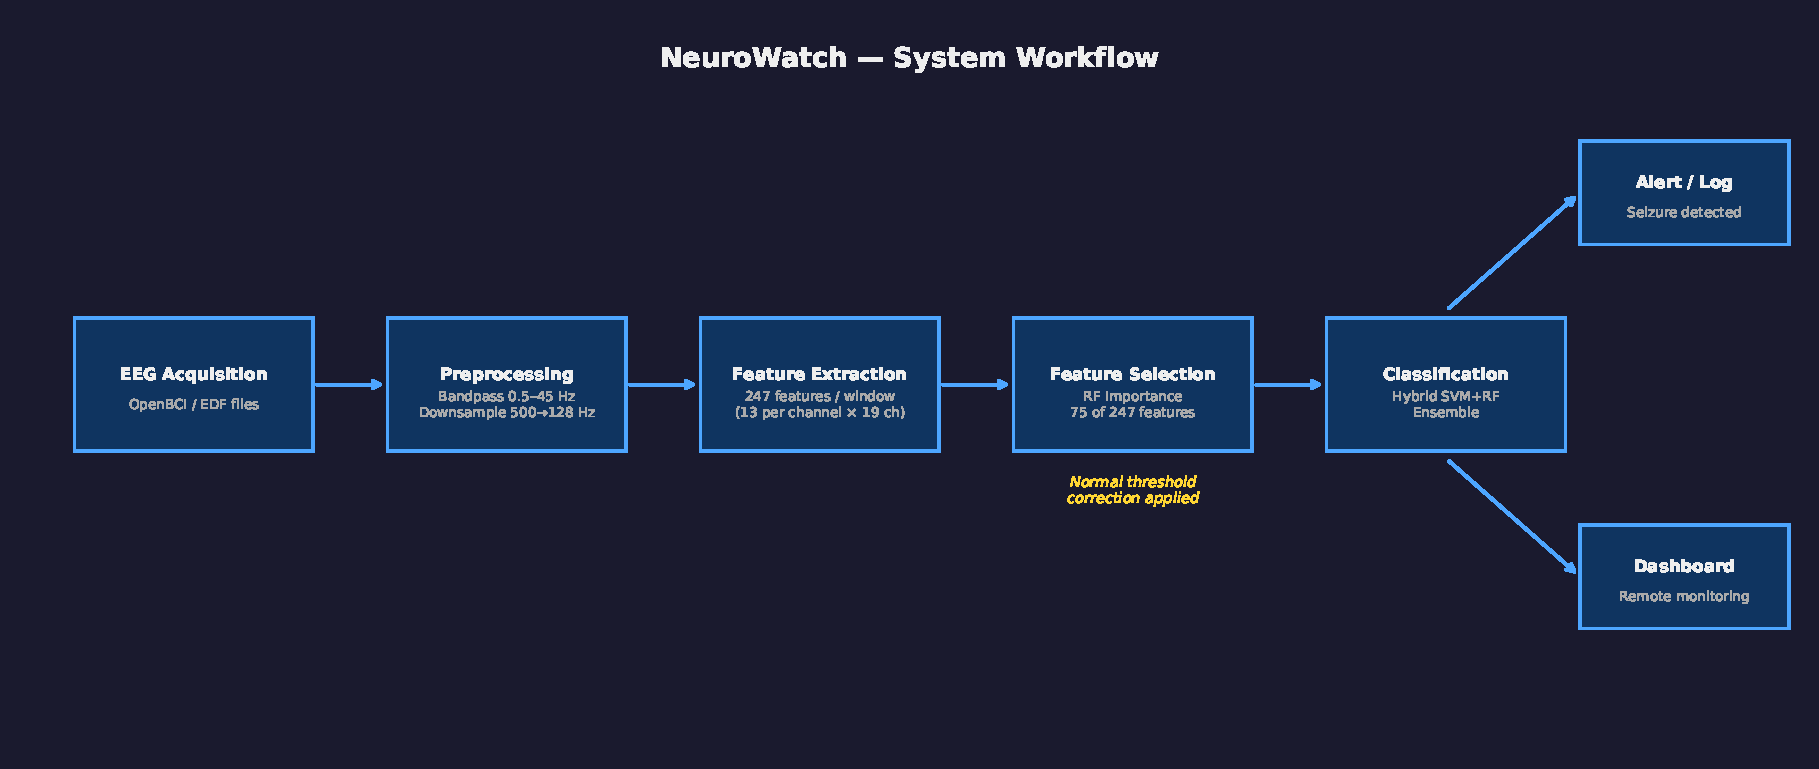
\includegraphics[width=\linewidth]{fig1_system_workflow}
  \caption{NeuroWatch end-to-end system workflow from EEG acquisition
           to alert generation and remote dashboard display.}
  \label{fig:workflow}
\end{figure}

\section{Dataset}

The classifier was trained and evaluated on the \textbf{Mendeley Focal
Epilepsy EEG Dataset}~\cite{mendeley_dataset}, which contains
continuous 19-channel EEG recordings from \textbf{six patients} undergoing
pre-surgical evaluation for drug-resistant focal epilepsy. Key dataset
characteristics are listed in Table~\ref{tab:dataset}.

\begin{table}[H]
  \centering
  \caption{Summary of the Mendeley Focal Epilepsy EEG Dataset.}
  \label{tab:dataset}
  \begin{tabular}{ll}
    \toprule
    \textbf{Property}          & \textbf{Value} \\
    \midrule
    Number of patients         & 6 (all focal epilepsy) \\
    EEG montage                & 19-channel international 10--20 \\
    Sampling rate              & 500~Hz \\
    Total recordings           & 20 EDF files \\
    Total annotated seizures   & 35 \\
    Longest seizure            & 86.3~s (Patient 12, Record 1) \\
    Original labelled NumPy windows & 7{,}790 (7{,}011 train + 779 test) \\
    Reconstructed modelling windows & 11{,}685 (9{,}348 train + 1{,}168 validation + 1{,}169 test) \\
    Window size                & 1~s (500 samples per channel before resampling) \\
    \bottomrule
  \end{tabular}
\end{table}

Medications were withdrawn prior to recording to facilitate ictal activity.
Seizure onset, offset, and type annotations were provided by the dataset
authors.

\subsection{Original Dataset vs Reconstructed Corpus}
\label{sec:original_vs_reconstructed}

The Mendeley Epileptic EEG Dataset is delivered as pre-processed NumPy
files, where each one-second window has been extracted from the raw EDF
recordings and assigned one of four labels: Normal, Complex Partial
Seizure (CPS), Electrographic Seizure, and Video-Detected Seizure. These
labels, summarised in Table~\ref{tab:mendeley_labels}, reflect the
seizure-type annotations from the original study. The files are split into
training and test sets: \texttt{x\_train.npy} contains 7{,}011 windows
and \texttt{x\_test.npy} contains 779 windows, summing to a total of
7{,}790 windows.

\begin{table}[H]
  \centering
  \caption{Class label definitions and segment counts in the original
           distributed Mendeley NumPy dataset.}
  \label{tab:mendeley_labels}
  \small
  \renewcommand{\arraystretch}{1.15}
  \begin{tabularx}{0.95\linewidth}{c>{\raggedright\arraybackslash}Xrr}
    \toprule
    \textbf{Label} & \textbf{Class} & \textbf{Segments} & \textbf{Duration (s)} \\
    \midrule
    0 & Normal & 3{,}895 & 3{,}895 \\
    1 & Complex Partial Seizure (CPS) & 3{,}034 & 3{,}034 \\
    2 & Electrographic Seizure & 750 & 750 \\
    3 & Video-Detected Seizure (no clear EEG visual change) & 111 & 111 \\
    \midrule
      & \textbf{Total} & \textbf{7{,}790} & \textbf{7{,}790} \\
    \bottomrule
  \end{tabularx}
\end{table}

\noindent While this structure is sufficient for binary seizure detection,
it presents a fundamental problem for pre-ictal classification because no
genuine pre-ictal class exists. The label described as ``Pre-Seizure'' in
some works derived from this corpus is simply a relabelling of CPS
activity---ongoing ictal or peri-ictal data---rather than a meaningful
warning window that precedes seizure onset. The Video-Detected category
captures events identified through observation rather than measurable EEG
change, introducing noise into any EEG-based classifier. Most importantly,
the pre-processed \texttt{.npy} files discard the continuous temporal
structure of the original recordings and replace it with fixed-length
segments assigned to broad categories. This means that exact seizure
timestamps, namely onset and offset times, which are needed to isolate a
genuine pre-ictal period, are lost entirely.

\subsubsection*{Reconstructing a Three-Class Pre-Ictal Corpus from Raw EDF}

For this reason, a separate reconstructed corpus was created directly from
the raw EDF recordings using a hand-curated seizure timestamp database
(\texttt{SEIZURE\_DB}). The pipeline loads each raw EDF file with
MNE-Python, preserving absolute start times and allowing seizure
wall-clock times to be converted into sample-level indices. Only
EEG-confirmed seizure timestamps are used; video-detected events are
excluded. For each confirmed seizure, three non-overlapping window types
are extracted, as shown in Table~\ref{tab:window_types}.

\begin{table}[H]
  \centering
  \caption{Window extraction scheme applied to each confirmed seizure event.}
  \label{tab:window_types}
  \small
  \renewcommand{\arraystretch}{1.15}
  \begin{tabularx}{0.95\linewidth}{>{\raggedright\arraybackslash}p{2.8cm}
                                  >{\raggedright\arraybackslash}X c}
    \toprule
    \textbf{Class} & \textbf{Temporal Window} & \textbf{Label} \\
    \midrule
    Normal & More than 60~min from any seizure onset or offset & 0 \\
    Pre-ictal & 5 to 30~min before seizure onset & 1 \\
    Ictal & Seizure onset to seizure offset & 2 \\
    \bottomrule
  \end{tabularx}
\end{table}

\noindent The pre-ictal window spans the interval from 30~minutes to
5~minutes before each seizure onset, giving a 25-minute segment that
reflects the transition period before a seizure. The five-minute buffer
between the window end and the onset marker ensures that no early ictal
discharges contaminate the pre-ictal label.

\subsubsection*{Temporal Safety Constraints}

Two safeguards prevent class contamination. First, when two seizures occur
in close succession, the pre-ictal window of the later seizure is clipped
so that it cannot overlap with the post-ictal recovery period of the
earlier seizure. This prevents post-ictal suppression or early
re-excitation from being mislabelled as pre-ictal activity. Second, Normal
windows are subject to a strict 60-minute exclusion zone on both sides of
every seizure. Any candidate Normal segment that falls within 60~minutes
of either the onset or offset of any seizure is discarded, ensuring that
interictal baseline windows are free from peri-ictal changes that could
otherwise bias the classifier.

\begin{table}[H]
  \centering
  \caption{Effect of the 60-minute Normal exclusion rule and subsequent
           balancing on segment counts.}
  \label{tab:normal_exclusion_effect}
  \footnotesize
  \setlength{\tabcolsep}{3pt}
  \renewcommand{\arraystretch}{1.2}
  \begin{tabularx}{\textwidth}{>{\raggedright\arraybackslash}p{3.4cm}
                              >{\centering\arraybackslash}p{1.5cm}
                              >{\centering\arraybackslash}p{1.6cm}
                              >{\centering\arraybackslash}p{1.3cm}
                              >{\centering\arraybackslash}p{1.5cm}
                              >{\raggedright\arraybackslash}X}
    \toprule
    \textbf{Processing stage} &
    \textbf{Normal} &
    \textbf{Pre-ictal} &
    \textbf{Ictal} &
    \textbf{Total} &
    \textbf{Interpretation} \\
    \midrule
    Before exclusion &
    165{,}015 & 39{,}227 & 3{,}895 & 208{,}137 &
    Candidate windows after removing ictal and pre-ictal intervals, before
    applying the Normal safety buffer. \\
    After exclusion &
    38{,}053 & 39{,}227 & 3{,}895 & 81{,}175 &
    The safety buffer removes 126{,}962 candidate Normal windows that are too
    close to seizure activity. \\
    Final balanced corpus &
    3{,}895 & 3{,}895 & 3{,}895 & 11{,}685 &
    Normal and Pre-ictal windows are subsampled to match the ictal count,
    preventing class domination during training. \\
    \bottomrule
  \end{tabularx}
\end{table}

\noindent Table~\ref{tab:normal_exclusion_effect} shows that the
60-minute exclusion rule substantially reduces the Normal candidate pool
before class balancing. This makes the Normal class more conservative:
only windows sufficiently distant from seizure activity are retained as
baseline examples.

\subsubsection*{Class Balancing and Final Dataset Composition}

Continuous recordings naturally produce far more interictal data than
ictal or pre-ictal data, so a subsampling step is applied after extraction.
All ictal windows are kept in full, while Normal and Pre-ictal windows are
capped at a fixed multiple of the ictal count. This prevents the Normal
class from dominating training and ensures that the model sees a balanced
representation of all three states. The final reconstructed corpus
contains 11{,}685 windows in the reported split: 9{,}348 training,
1{,}168 validation, and 1{,}169 test windows. The arrays are saved as
\texttt{x\_train.npy}, \texttt{y\_train.npy}, \texttt{x\_val.npy},
\texttt{y\_val.npy}, \texttt{x\_test.npy}, and \texttt{y\_test.npy}
under the \texttt{Npy\_files\_preictal/} directory. Thus, 7{,}790 refers
to the original four-class NumPy dataset, while 11{,}685 is the
reconstructed EDF-based three-class corpus used for model training and
evaluation.

Table~\ref{tab:dataset_comparison} summarises the limitations of the
original dataset alongside the corresponding fixes applied in the
reconstructed corpus.

\begin{table}[H]
  \centering
  \caption{Comparison between the original distributed dataset and the
           reconstructed pre-ictal corpus.}
  \label{tab:dataset_comparison}
  \small
  \renewcommand{\arraystretch}{1.2}
  \begin{tabularx}{\textwidth}{>{\raggedright\arraybackslash}X
                              >{\raggedright\arraybackslash}X}
    \toprule
    \textbf{Limitation of Original Dataset} &
    \textbf{Resolution in Reconstructed Corpus} \\
    \midrule
    No genuine pre-ictal class; the ``Pre-Seizure'' label reflects ongoing CPS activity &
    Pre-ictal windows are extracted strictly from the 5 to 30~minute period before confirmed onset \\
    Video-Detected category includes events with no measurable EEG signature &
    Video-detected events are excluded; only EEG-confirmed seizure timestamps are used \\
    Pre-processed \texttt{.npy} files discard continuous temporal structure &
    Raw EDF recordings are loaded directly, preserving absolute timestamps \\
    Normal segments may contain peri-ictal neurophysiology &
    A 60-minute exclusion buffer on both sides of every seizure enforces clean Normal windows \\
    No handling of closely spaced seizures &
    The pre-ictal window is clipped to the post-ictal boundary of any preceding seizure \\
    \bottomrule
  \end{tabularx}
\end{table}

\section{Preprocessing}
\label{sec:preprocessing}

Figure~\ref{fig:sigproc} illustrates the preprocessing stages applied
to each raw EEG signal before feature extraction.

\begin{figure}[H]
  \centering
  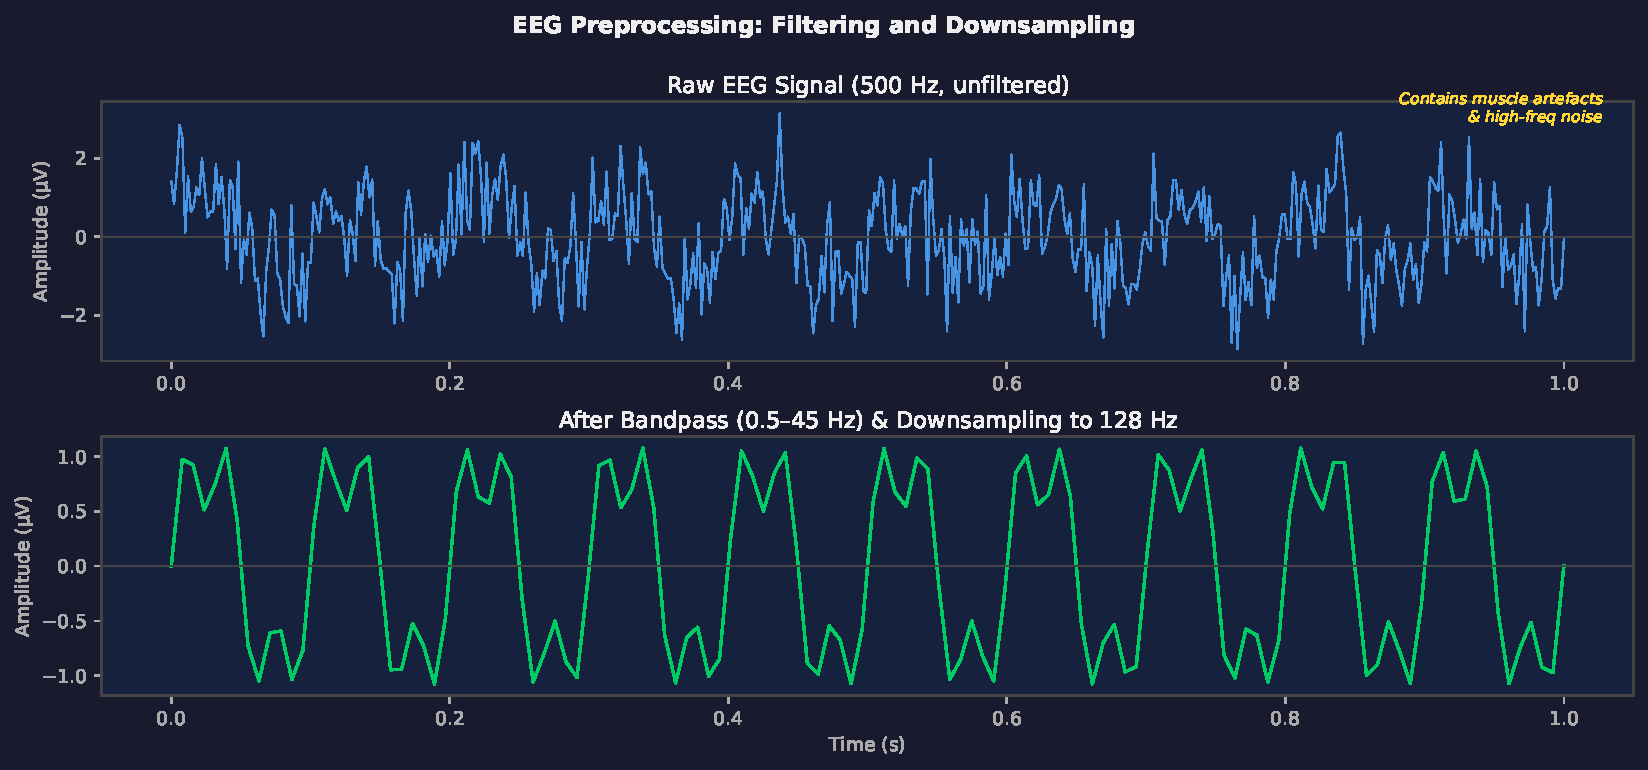
\includegraphics[width=\linewidth]{fig3_signal_processing}
  \caption{Comparison of a raw 500~Hz EEG trace (top) and the same signal
           after 4th-order Butterworth bandpass filtering (0.5--45~Hz)
           and downsampling to 128~Hz (bottom).}
  \label{fig:sigproc}
\end{figure}

\subsection{Bandpass Filtering}

A \textbf{4th-order zero-phase Butterworth bandpass filter} is applied
over the frequency range $[0.5,\,45]$~Hz to suppress DC drift and
high-frequency muscle artefacts while preserving the relevant
EEG rhythms ($\delta$, $\theta$, $\alpha$, $\beta$, and lower $\gamma$).
Zero-phase filtering is achieved by applying the filter forwards and
backwards (\texttt{scipy.signal.filtfilt}), eliminating phase distortion.

The transfer function of an $N$th-order Butterworth filter is defined by
its magnitude response:
\begin{equation}
  |H(j\omega)|^2 = \frac{1}{1+\left(\dfrac{\omega}{\omega_c}\right)^{2N}}
  \label{eq:butterworth}
\end{equation}
where $\omega_c$ is the cut-off angular frequency and $N=4$.

\subsection{Downsampling}

After filtering, each channel is resampled from 500~Hz to \textbf{128~Hz}
using \texttt{scipy.signal.resample}.
This reduces the number of time-domain samples per channel from 500 to
128 samples per one-second window, lowering computational
cost while remaining above the Nyquist rate for all retained frequencies.

\subsection{Window Tiling}

Because Welch's method requires a minimum window length, each resampled
signal is tiled to exactly \textbf{4{,}097 samples} (approximately
32~seconds equivalent at 128~Hz) by repeating the signal as necessary,
then truncating. Welch's method is subsequently applied with
\texttt{nperseg=128}, yielding a frequency resolution of exactly 1~Hz.

\subsection{Artefact Handling}

The preprocessing pipeline uses filtering and consistent channel handling,
but it does not apply independent component analysis (ICA), EOG/EMG
regression, or automatic amplitude-threshold rejection. This decision keeps
the training and inference pipelines identical and reproducible on the
Raspberry Pi, but it also means that residual ocular, movement, and muscle
artefacts may remain in some windows. The operational artefact handling is
summarised in Table~\ref{tab:artefact_handling}.

\begin{table}[H]
  \centering
  \caption{Artefact handling used in the implemented preprocessing pipeline.}
  \label{tab:artefact_handling}
  \footnotesize
  \renewcommand{\arraystretch}{1.18}
  \begin{tabularx}{\textwidth}{>{\raggedright\arraybackslash}p{3.5cm}
                              >{\raggedright\arraybackslash}p{4.2cm}
                              >{\raggedright\arraybackslash}X}
    \toprule
    \textbf{Artefact source} & \textbf{Operational handling} & \textbf{Limitation} \\
    \midrule
    DC drift and slow baseline movement &
    0.5~Hz high-pass component of the Butterworth bandpass filter &
    Very slow non-stationary changes may still affect the one-second window. \\
    Powerline and high-frequency noise &
    45~Hz low-pass component; the retained band excludes 50~Hz powerline
    interference &
    No separate adaptive notch filter is applied during model inference. \\
    Muscle artefacts and movement noise &
    High-frequency components above 45~Hz are attenuated &
    Low-frequency movement artefacts can remain if they fall inside the
    retained EEG band. \\
    Ocular artefacts &
    No ICA, EOG channel regression, or blink-specific removal is applied &
    This is a limitation of the implemented system and may affect windows
    containing strong eye movements. \\
    Bad or inconsistent channels &
    The reconstructed corpus uses a consistent 19-channel montage &
    No automatic per-window channel rejection is performed. \\
    Amplitude outliers &
    Max-absolute normalisation is applied before feature extraction &
    Amplitude threshold rejection is not used; abnormal windows are scaled
    rather than discarded. \\
    \bottomrule
  \end{tabularx}
\end{table}

\subsection{Normalisation Consistency}

Three separate normalisation steps are used for different purposes. Raw EDF
windows are max-absolute normalised before feature extraction in both the
reconstructed training corpus and the live inference code. Relative band-power
normalisation is then applied inside the spectral feature calculation. Finally,
\texttt{StandardScaler} is fitted on training features only and is used for
the SVM branch; the RF branch receives the same selected features without
feature scaling.

\begin{table}[H]
  \centering
  \caption{Normalisation controls used to reduce train--inference mismatch.}
  \label{tab:normalisation_controls}
  \footnotesize
  \renewcommand{\arraystretch}{1.18}
  \begin{tabularx}{\textwidth}{>{\raggedright\arraybackslash}p{3.4cm}
                              >{\raggedright\arraybackslash}p{4.3cm}
                              >{\raggedright\arraybackslash}X}
    \toprule
    \textbf{Stage} & \textbf{Where applied} & \textbf{Purpose} \\
    \midrule
    Max-absolute raw-window scaling &
    EDF reconstruction and live inference before feature extraction &
    Places raw amplitudes on a comparable scale so that inference windows
    follow the same preprocessing assumption as the saved training windows. \\
    Relative band-power scaling &
    During Welch band-power extraction &
    Uses the proportion of power in each band rather than absolute amplitude,
    reducing sensitivity to recording gain differences. \\
    Training-set \texttt{StandardScaler} &
    Fitted on training features only; applied to validation, test, and
    inference features for SVM &
    Prevents data leakage and gives the RBF SVM a stable feature scale. \\
    RF unscaled feature branch &
    RF receives selected features without \texttt{StandardScaler} &
    Maintains the scale-invariant tree behaviour of Random Forest. \\
    \bottomrule
  \end{tabularx}
\end{table}

The implementation therefore does not apply a different mathematical
normalisation at inference; instead, inference repeats the raw-window
max-absolute scaling already used when reconstructing the training corpus.
A formal distribution-shift plot comparing live hardware recordings with
the reconstructed corpus was not produced, and this remains a limitation
for future validation.

\section{Feature Extraction}
\label{sec:features}

Figure~\ref{fig:featpipeline} illustrates how 13 scalar features are
computed from each EEG channel, resulting in a
$19 \times 13 = \mathbf{247}$-dimensional feature vector per window.

\begin{figure}[H]
  \centering
  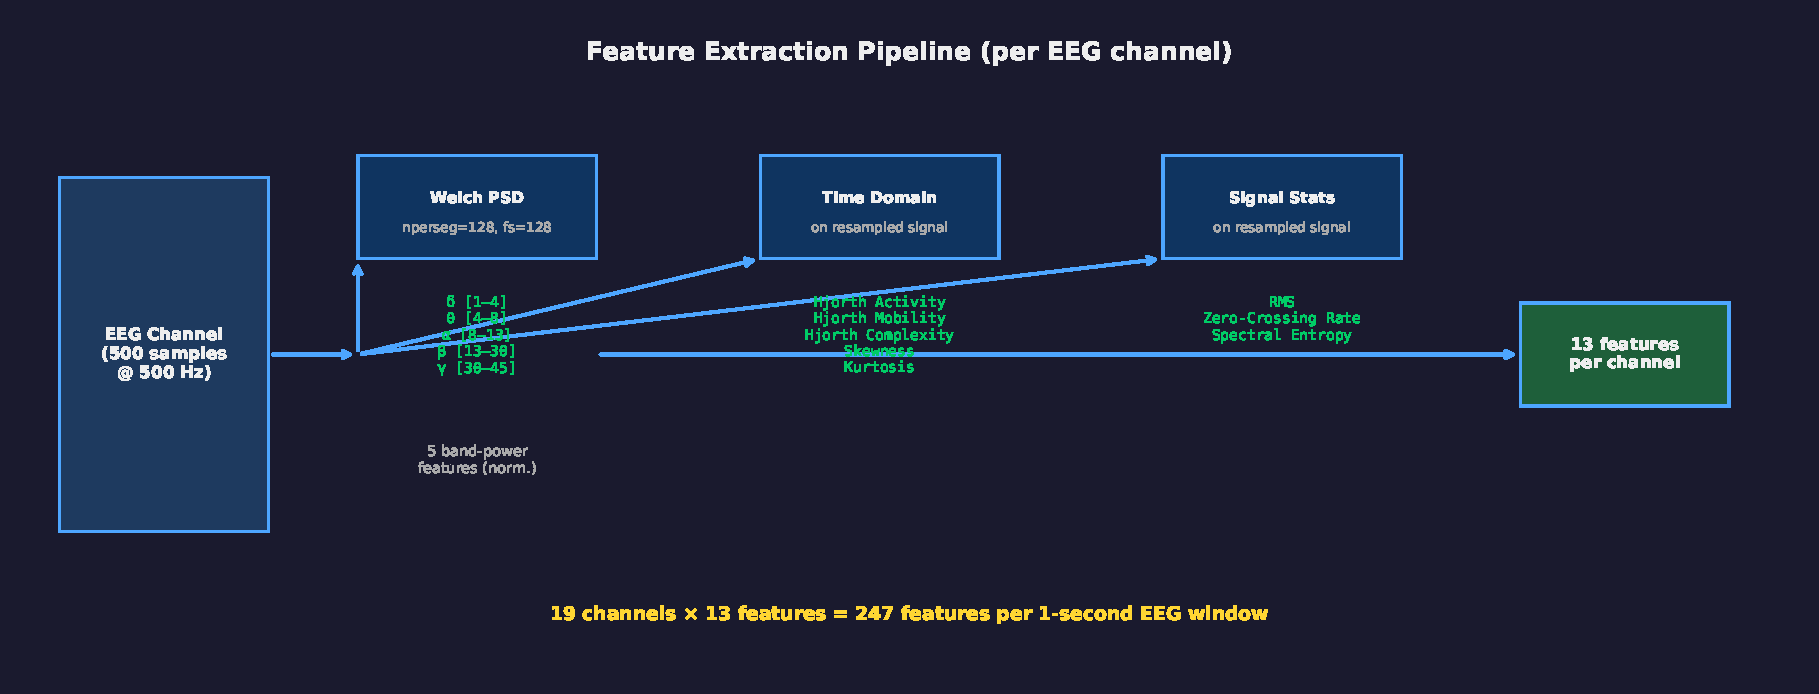
\includegraphics[width=\linewidth]{fig2_feature_pipeline}
  \caption{Feature extraction pipeline applied independently to each of
           the 19 EEG channels. The 13 per-channel features are
           concatenated to form the 247-dimensional feature vector.}
  \label{fig:featpipeline}
\end{figure}

Table~\ref{tab:feature_list} lists the exact 13 features extracted from
each channel. Since spectral entropy is included as the thirteenth feature,
the total remains mathematically consistent:
\[
19\ \text{channels} \times 13\ \text{features per channel} = 247.
\]

\begin{table}[H]
  \centering
  \caption{Exact per-channel features used to form the 247-dimensional vector.}
  \label{tab:feature_list}
  \footnotesize
  \renewcommand{\arraystretch}{1.15}
  \begin{tabularx}{\textwidth}{>{\centering\arraybackslash}p{1.0cm}
                              >{\raggedright\arraybackslash}p{3.6cm}
                              >{\raggedright\arraybackslash}X}
    \toprule
    \textbf{No.} & \textbf{Feature} & \textbf{Description} \\
    \midrule
    1 & Delta relative band power & Mean Welch PSD power in 1--4~Hz, divided by total band power. \\
    2 & Theta relative band power & Mean Welch PSD power in 4--8~Hz, divided by total band power. \\
    3 & Alpha relative band power & Mean Welch PSD power in 8--13~Hz, divided by total band power. \\
    4 & Beta relative band power & Mean Welch PSD power in 13--30~Hz, divided by total band power. \\
    5 & Gamma relative band power & Mean Welch PSD power in 30--45~Hz, divided by total band power. \\
    6 & Hjorth activity & Signal variance. \\
    7 & Hjorth mobility & Square root of derivative variance divided by signal variance. \\
    8 & Hjorth complexity & Ratio of derivative mobility to signal mobility. \\
    9 & Skewness & Third standardised moment of the signal. \\
    10 & Excess kurtosis & Fourth standardised moment minus 3. \\
    11 & Root mean square & Quadratic mean signal amplitude. \\
    12 & Zero-crossing rate & Proportion of adjacent samples with a sign change. \\
    13 & Spectral entropy & Normalised entropy of the Welch power spectrum. \\
    \bottomrule
  \end{tabularx}
\end{table}

\subsection{Band-Power Features (5 per channel)}

Band power is estimated using Welch's periodogram. The Power Spectral
Density (PSD) $S(f)$ is integrated over five standard EEG frequency
bands:
\begin{align}
  P_\delta &= \overline{S(f)},\quad f \in [1, 4]~\text{Hz} \notag\\
  P_\theta &= \overline{S(f)},\quad f \in [4, 8]~\text{Hz} \notag\\
  P_\alpha &= \overline{S(f)},\quad f \in [8, 13]~\text{Hz} \notag\\
  P_\beta  &= \overline{S(f)},\quad f \in [13, 30]~\text{Hz} \notag\\
  P_\gamma &= \overline{S(f)},\quad f \in [30, 45]~\text{Hz} \notag
\end{align}

To remove the confounding effect of absolute signal amplitude, each
band-power vector is \textbf{normalised} to sum to unity:
\begin{equation}
  \tilde{P}_k = \frac{P_k}{\displaystyle\sum_{j=1}^{5} P_j + \varepsilon},
  \quad k \in \{\delta, \theta, \alpha, \beta, \gamma\}
  \label{eq:bpnorm}
\end{equation}
where $\varepsilon = 10^{-10}$ guards against division by zero.

\subsection{Hjorth Parameters (3 per channel)}

Hjorth parameters~\cite{hjorth1970eeg} describe the statistical properties
of the signal in the time domain. Let $x(n)$, $x'(n)$, and $x''(n)$
denote the signal, its first difference, and second difference,
respectively.

\begin{align}
  \text{Activity}   &= \sigma^2_x \label{eq:hjorth_act} \\[4pt]
  \text{Mobility}   &= \sqrt{\frac{\sigma^2_{x'}}{\sigma^2_x}}
                      \label{eq:hjorth_mob} \\[4pt]
  \text{Complexity} &= \frac{\text{Mobility}(x')}{\text{Mobility}(x)}
                      = \sqrt{\frac{\sigma^2_{x''}\,\sigma^2_x}{\left(\sigma^2_{x'}\right)^2}}
                      \label{eq:hjorth_comp}
\end{align}

Activity reflects signal power; Mobility approximates the mean frequency;
Complexity measures the similarity of the signal's shape to a sine wave.

\subsection{Higher-Order Statistics (2 per channel)}

\textbf{Skewness} and \textbf{excess kurtosis} capture the asymmetry and
tail-heaviness of the amplitude distribution:
\begin{equation}
  \text{Skewness} = \frac{\mu_3}{\sigma^3}, \qquad
  \text{Kurtosis} = \frac{\mu_4}{\sigma^4} - 3
  \label{eq:highorder}
\end{equation}
where $\mu_k = \mathbb{E}[(x - \bar{x})^k]$ is the $k$th central moment.

\subsection{Root Mean Square (1 per channel)}

RMS quantifies the overall signal energy:
\begin{equation}
  x_{\text{RMS}} = \sqrt{\frac{1}{N}\sum_{n=1}^{N} x(n)^2}
  \label{eq:rms}
\end{equation}

\subsection{Zero-Crossing Rate (1 per channel)}

ZCR measures how rapidly the signal changes sign, serving as a
frequency-domain proxy without spectral computation:
\begin{equation}
  \text{ZCR} = \frac{1}{N-1}\sum_{n=1}^{N-1}
               \mathbf{1}\!\left[x(n)\cdot x(n+1) < 0\right]
  \label{eq:zcr}
\end{equation}

\subsection{Spectral Entropy (1 per channel)}

Spectral entropy measures the uniformity of the PSD. A flat (white-noise)
spectrum maximises entropy; a narrow-band signal minimises it:
\begin{equation}
  H_{\text{spec}} = -\frac{\displaystyle\sum_{k} \tilde{p}_k \log_2(\tilde{p}_k + \varepsilon)}
                          {\log_2(M + 1)}
  \label{eq:specent}
\end{equation}
where $\tilde{p}_k = S(f_k)/(\sum_j S(f_j) + \varepsilon)$ is the
normalised PSD and $M$ is the number of frequency bins.

\section{Feature Selection}
\label{sec:selection}

Of the 247 raw features, \textbf{75} are selected using a
\textit{bootstrap Random Forest importance ranking}. In this stage, the
RF is used specifically for \textbf{feature ranking and feature selection},
not for final classification. A separate Random Forest with 300 trees and
\texttt{max\_depth=10} is trained on the full feature set. Each tree votes
on a random subset of features; the mean
decrease in Gini impurity attributable to feature $i$ is accumulated
across all trees:
\begin{equation}
  \hat{\phi}_i =
  \frac{1}{T}\sum_{t=1}^{T}\sum_{v\in t:\,\text{split on }i}
  \Delta G(v)
  \label{eq:rfimportance}
\end{equation}
where $T=300$ is the number of trees and $\Delta G(v)$ is the impurity
decrease at node $v$. Features are ranked by $\hat{\phi}_i$ in descending
order and the top 75 indices are retained and sorted to preserve their
original relative ordering:
\begin{equation}
  \mathcal{S} = \text{sort}\!\left(\underset{i}{\mathrm{argtop}}_{75}\,\hat{\phi}_i\right)
  \label{eq:topk}
\end{equation}
The index set $\mathcal{S}$ is saved with the trained scaler and classifier
artefacts so that identical feature slicing can be reproduced at inference
time.

The value of 75 selected features is therefore not arbitrary: it is the
selected operating point of the implemented RF-importance pipeline. However,
a complete top-$k$ ablation over 25, 50, 75, 100, and 247 features was not
fully retained as a reproducible experiment log. Table~\ref{tab:feature_ablation_status}
therefore distinguishes between the implemented final configuration and the
additional ablations that should be included in a future extended evaluation.

\begin{table}[H]
  \centering
  \caption{Feature-selection evaluation status for the proposed model.}
  \label{tab:feature_ablation_status}
  \footnotesize
  \renewcommand{\arraystretch}{1.18}
  \begin{tabularx}{\textwidth}{>{\centering\arraybackslash}p{1.4cm}
                              >{\raggedright\arraybackslash}p{4.0cm}
                              >{\raggedright\arraybackslash}X}
    \toprule
    \textbf{Features} & \textbf{Evaluation status} & \textbf{Interpretation} \\
    \midrule
    25 & Not retained in the final experiment log &
    Would test whether a very compact feature set preserves seizure recall. \\
    50 & Not retained in the final experiment log &
    Would test whether moderate compression is sufficient. \\
    75 & Final implemented setting &
    Selected by RF importance ranking and used in the RF60+SVM40\_C2 model. \\
    100 & Not retained in the final experiment log &
    Would test whether adding lower-ranked features improves accuracy or
    introduces noise. \\
    247 & Full-feature reference required for future ablation &
    Would measure whether feature selection improves generalisation relative
    to using every extracted feature. \\
    \bottomrule
  \end{tabularx}
\end{table}

Consequently, the reported final model is justified operationally by the
saved RF-importance selector and held-out validation performance, while a
full feature-count ablation remains a recommended extension for stronger
experimental evidence.

\section{Classification: SVM and Random Forest}
\label{sec:classification}

\subsection{Support Vector Machine}

An SVM with an RBF (Gaussian) kernel is trained on the
\textbf{StandardScaler-normalised} and feature-selected data. The primal
optimisation problem for the soft-margin SVM is:
\begin{equation}
  \min_{\mathbf{w},\,b,\,\boldsymbol{\xi}}\;
  \frac{1}{2}\|\mathbf{w}\|^2 + C\sum_{i=1}^{n}\xi_i
  \label{eq:svm_primal}
\end{equation}
subject to $y_i(\mathbf{w}^\top\phi(\mathbf{x}_i)+b)\geq 1-\xi_i$ and
$\xi_i\geq 0$. The regularisation parameter is set to $C=2$, balancing
margin width against training error.

The RBF kernel is:
\begin{equation}
  K(\mathbf{x}_i,\mathbf{x}_j) = \exp\!\left(-\gamma\|\mathbf{x}_i-\mathbf{x}_j\|^2\right)
  \label{eq:rbf}
\end{equation}
with $\gamma = 1/(\text{n\_features}\cdot\sigma^2_X)$ (\texttt{scale}
setting).

Because this project addresses a three-class problem
(\textit{Normal}, \textit{Pre-Seizure}, and \textit{Seizure}), the SVM is
not used as a single binary classifier. The implementation uses
\texttt{sklearn.svm.SVC} with the RBF kernel, which handles multiclass
classification through a one-vs-one strategy. For $K=3$ classes, this
trains $\frac{K(K-1)}{2}=3$ binary decision functions: Normal versus
Pre-Seizure, Normal versus Seizure, and Pre-Seizure versus Seizure. The
pairwise decision outputs are combined internally to produce a final
three-class decision, and probability calibration is then used to obtain
$\mathbf{p}_{\text{SVM}} = [p_0, p_1, p_2]$.

The regularisation parameter $C$ controls the trade-off between maximising
the margin and penalising training errors. In this project, $C$ was tuned
empirically by comparing validation performance for candidate values. The
final model uses $C=2$, which improved the validation and test performance
relative to the earlier $C=1$ configuration while keeping the overfitting
gap within an acceptable range. The kernel width parameter $\gamma$ was
set to \texttt{scale}, meaning that scikit-learn computes
$\gamma = 1/(p\,\mathrm{Var}(X))$, where $p$ is the number of selected
features and $\mathrm{Var}(X)$ is the variance of the scaled training
data. This automatic setting adapts the RBF width to the feature scale
after StandardScaler normalisation, avoiding a manually fixed $\gamma$
that may be too narrow or too broad for the selected EEG feature space.

Class imbalance in the pre-ictal class is addressed through asymmetric
penalty weights:
\begin{equation}
  \mathbf{c} = \{0:\,1.0,\;\; 1:\,1.8,\;\; 2:\,1.0\}
  \label{eq:classweight}
\end{equation}
which penalises misclassification of Pre-Seizure samples 1.8$\times$
more than Normal or Seizure.

Probability outputs are obtained via Platt scaling, fitting a sigmoid
$\sigma(\alpha\,f(\mathbf{x})+\beta)$ to the decision values using
5-fold cross-validation within the training set
(\texttt{probability=True}).

\subsection{Project-Specific Role of Support Vector Machine}
\label{sec:svm_project_role}

In this project, SVM is used specifically as a \textbf{classification model}
in the final hybrid ensemble. Unlike RF, SVM is not used for feature
selection. The feature subset is first chosen by the RF importance selector,
then the SVM receives the \textbf{StandardScaler-normalised} version of
those selected features. Its role is to learn a refined nonlinear decision
boundary between Normal, Pre-Seizure, and Seizure EEG windows using the RBF
kernel. The SVM outputs a class-probability vector
$\mathbf{p}_{\text{SVM}}$, which contributes \textbf{40\%} to the final
ensemble probability.

\begin{table}[H]
  \centering
  \caption{Specific Support Vector Machine role in the proposed implementation.}
  \label{tab:svm_role}
  \footnotesize
  \setlength{\tabcolsep}{3pt}
  \renewcommand{\arraystretch}{1.2}
  \begin{tabularx}{\textwidth}{>{\raggedright\arraybackslash}p{2.5cm}
                              >{\raggedright\arraybackslash}p{3.1cm}
                              >{\raggedright\arraybackslash}X
                              >{\raggedright\arraybackslash}X}
    \toprule
    \textbf{SVM usage} & \textbf{Pipeline location} & \textbf{Input and output} & \textbf{Purpose} \\
    \midrule
    Classification contribution &
    Final hybrid ensemble classifier &
    Input: scaled and RF-selected EEG features. Output: SVM class probabilities
    $\mathbf{p}_{\text{SVM}}$ for Normal, Pre-Seizure, and Seizure. &
    Learns an RBF-kernel decision boundary and contributes \textbf{40\%}
    of the final ensemble probability before threshold correction. \\
    \bottomrule
  \end{tabularx}
\end{table}

\subsection{Random Forest}

A Random Forest is also used as a \textbf{classifier} in the final hybrid
ensemble. This is separate from the earlier RF importance selector:
the selector ranks and keeps features, while the classifier produces
class probabilities for Normal, Pre-Seizure, and Seizure. A Random Forest
of 500 classification trees is trained on the feature-selected but
\textbf{unscaled} data. Each tree $t$ is grown on a bootstrap resample
$\mathcal{B}_t \sim D$ with replacement. At each
node the best split is chosen over a random subset of
$\lceil\sqrt{p}\rceil$ features by maximising the Gini impurity reduction:
\begin{equation}
  \Delta G = G_{\text{parent}}
             - \frac{n_L}{n}G_L
             - \frac{n_R}{n}G_R
  \label{eq:gini}
\end{equation}
\begin{equation}
  G = 1 - \sum_{k=0}^{K-1} p_k^2
  \label{eq:gini_def}
\end{equation}
where $p_k$ is the fraction of class-$k$ samples at the node, $K=3$.
Structural regularisation uses \texttt{max\_depth=5} and
\texttt{min\_samples\_leaf=10}. Class balance is enforced via
\texttt{class\_weight="balanced"}, which sets:
\begin{equation}
  w_k = \frac{n}{K \cdot n_k}
  \label{eq:rf_classweight}
\end{equation}

Per-tree probability estimates are averaged over all trees to give the
RF probability vector $\mathbf{p}_{\text{RF}}$, which contributes
\textbf{60\%} of the final ensemble probability.

\subsection{Project-Specific Role of Random Forest}
\label{sec:rf_project_role}

In this project, RF is not used only as a generally ``robust'' algorithm.
It has two explicit and separate responsibilities in the implemented
pipeline. First, RF is used for \textbf{feature ranking and selection}:
the \texttt{RFImportanceSelector} ranks the 247 handcrafted EEG features
and retains the 75 most informative features. Second, RF is used as a
\textbf{classification model}: a separate RF classifier produces
$\mathbf{p}_{\text{RF}}$, the class-probability vector that contributes
60\% to the final ensemble prediction. These two RF components are saved
as different artefacts and are used at different points in the inference
pipeline, as summarised in Table~\ref{tab:rf_roles}.

\begin{table}[H]
  \centering
  \caption{Distinct Random Forest roles in the proposed implementation.}
  \label{tab:rf_roles}
  \footnotesize
  \setlength{\tabcolsep}{3pt}
  \renewcommand{\arraystretch}{1.2}
  \begin{tabularx}{\textwidth}{>{\raggedright\arraybackslash}p{2.5cm}
                              >{\raggedright\arraybackslash}p{3.1cm}
                              >{\raggedright\arraybackslash}X
                              >{\raggedright\arraybackslash}X}
    \toprule
    \textbf{RF usage} & \textbf{Pipeline location} & \textbf{Input and output} & \textbf{Purpose} \\
    \midrule
    Feature ranking and selection &
    \texttt{RFImportanceSelector} during training and inference &
    Input: 247 extracted EEG features. Output: 75 selected feature indices and reduced feature matrix. &
    Reduces dimensionality, removes weaker features, and ensures the SVM/RF classifiers receive the same selected feature subset. \\
    \midrule
    Classification contribution &
    Final hybrid ensemble classifier &
    Input: selected unscaled EEG features. Output: RF class probabilities
    $\mathbf{p}_{\text{RF}}$ for Normal, Pre-Seizure, and Seizure. &
    Contributes \textbf{60\%} of the final ensemble probability before the argmax decision and threshold correction. \\
    \bottomrule
  \end{tabularx}
\end{table}

This distinction is important because the first RF model is a selector,
whereas the second RF model is a classifier. The selector is stored as
\texttt{selector.pkl}; the classifier is stored as \texttt{rf\_model.pkl}.
During inference, \texttt{selector.pkl} is applied before classification,
while \texttt{rf\_model.pkl} participates directly in the ensemble
probability calculation.

\section{Ensemble Combination and Threshold Correction}
\label{sec:ensemble}

Figure~\ref{fig:architecture} shows the complete ensemble architecture.

\begin{figure}[H]
  \centering
  
\includegraphics[
    width=0.82\textwidth,
    height=0.58\textheight,
    keepaspectratio
  ]{fig4_model_architecture}
  \caption{Architecture of the proposed hybrid ensemble classifier.
           SVM and RF probability vectors are combined with fixed weights
           (40\% SVM, 60\% RF) and a post-hoc threshold correction
           suppresses false Pre-Seizure predictions.}
  \label{fig:architecture}
\end{figure}

\subsection{Weighted Probability Combination}

The final combined probability vector for a window $\mathbf{x}$ is:
\begin{equation}
  \mathbf{p}_{\text{combined}} =
  \alpha\,\mathbf{p}_{\text{SVM}}(\mathbf{x})
  + (1-\alpha)\,\mathbf{p}_{\text{RF}}(\mathbf{x}),
  \quad \alpha = 0.40
  \label{eq:ensemble}
\end{equation}
The weights $\alpha=0.40$ (SVM) and $1-\alpha=0.60$ (RF) were selected by
grid-searching the validation set over the range $\alpha \in [0.0, 1.0]$
in steps of 0.05. Thus, in the final classifier, RF is not only used for
feature selection; it also contributes the larger share, \textbf{60\%},
of the ensemble probability.

\begin{table}[H]
  \centering
  \caption{Validation-based ensemble weight selection.}
  \label{tab:ensemble_weight_selection}
  \footnotesize
  \renewcommand{\arraystretch}{1.18}
  \begin{tabularx}{\textwidth}{>{\centering\arraybackslash}p{2.2cm}
                              >{\centering\arraybackslash}p{2.2cm}
                              >{\raggedright\arraybackslash}p{3.4cm}
                              >{\raggedright\arraybackslash}X}
    \toprule
    \textbf{SVM weight} & \textbf{RF weight} & \textbf{Selection outcome} & \textbf{Reason} \\
    \midrule
    0.70 & 0.30 & Tested, not selected &
    Places most emphasis on the RBF SVM and reduces the stabilising effect
    of the RF probability estimate. \\
    0.60 & 0.40 & Tested, not selected &
    Gives SVM a majority contribution, but did not provide the selected
    validation operating point. \\
    0.50 & 0.50 & Tested, not selected &
    Equal weighting was considered as a neutral baseline. \\
    \textbf{0.40} & \textbf{0.60} & \textbf{Selected final setting} &
    Chosen by validation grid search; RF therefore contributes 60\% of the
    ensemble probability and SVM contributes 40\%. \\
    \bottomrule
  \end{tabularx}
\end{table}

\subsection{Normal Threshold Correction}

After the initial argmax prediction, a \textit{Normal threshold correction}
is applied to suppress false Pre-Seizure alarms:
\begin{equation}
  \hat{y} = \begin{cases}
    \text{Normal}     & \text{if } \hat{y}_0 = \text{Pre-Seizure and }
                        p_{\text{Normal}} \geq \theta \\
    \hat{y}_0         & \text{otherwise}
  \end{cases}
  \label{eq:threshold}
\end{equation}
The threshold $\theta$ is tuned on the validation set by a one-dimensional
grid search over $[0.30,\, 0.65]$ in steps of $0.01$, maximising overall
accuracy. Crucially, the correction is \textit{never} applied when the raw
prediction is Seizure, ensuring that true seizure recall is unaffected.
In the final RF60+SVM40\_C2 model, this correction is retained as part of
the implemented decision rule rather than treated as a rejected method. The
saved threshold value is $\theta=0.39$.

\subsection{Final Prediction Pipeline}

The complete per-window inference procedure is:

\begin{enumerate}[label=\arabic*.]
  \item Extract 247 features (Section~\ref{sec:features}).
  \item Apply feature selector $\mathcal{S}$, retaining 75 features.
  \item Normalise with the training-set \texttt{StandardScaler}:
        $\tilde{\mathbf{x}} = (\mathbf{x} - \boldsymbol{\mu}) / \boldsymbol{\sigma}$.
  \item Compute $\mathbf{p}_{\text{SVM}}$ from the scaled features.
  \item Compute $\mathbf{p}_{\text{RF}}$ from the \emph{unscaled} selected features.
  \item Blend: $\mathbf{p} = 0.40\,\mathbf{p}_{\text{SVM}} + 0.60\,\mathbf{p}_{\text{RF}}$.
  \item $\hat{y}_0 = \arg\max_k\, p_k$.
  \item If $\hat{y}_0 = \text{Pre-Seizure}$ and $p_{\text{Normal}} \geq \theta$,
        set $\hat{y} = \text{Normal}$; else $\hat{y} = \hat{y}_0$.
  \item Return $\hat{y}$ and $\max_k\, p_k$ as the confidence score.
\end{enumerate}

\section{Training Procedure}

\subsection{Data Split}

The balanced 11{,}685-sample dataset is divided into three non-overlapping
stratified splits using \texttt{train\_test\_split} with \texttt{random\_state=42}:

\begin{center}
  \begin{tabular}{lcc}
    \toprule
    \textbf{Split} & \textbf{Fraction} & \textbf{Samples} \\
    \midrule
    Training       & 80\%              & 9{,}348 \\
    Validation     & 10\%              & 1{,}168 \\
    Test           & 10\%              & 1{,}169 \\
    \bottomrule
  \end{tabular}
\end{center}

Stratification ensures each split contains equal proportions of all three
classes.

This 80/10/10 split applies only to the reconstructed EDF-based
three-class corpus used for the final experiments. It should not be
confused with the original distributed Mendeley NumPy files, which use a
90/10 train--test split of 7{,}011 and 779 one-second windows. The two
splits refer to different datasets: the original four-class labelled
dataset and the reconstructed three-class Pre-Seizure corpus.

\subsection{Hyper-parameter Summary}

\begin{table}[H]
  \centering
  \caption{Final hyper-parameter configuration for the RF60+SVM40\_C2 model.}
  \label{tab:hyperparams}
  \begin{tabular}{lll}
    \toprule
    \textbf{Component} & \textbf{Parameter} & \textbf{Value} \\
    \midrule
    \multirow{4}{*}{SVM}
      & Kernel              & RBF \\
      & $C$                 & 2 \\
      & $\gamma$            & scale \\
      & Class weights       & $\{0:1.0,\;1:1.8,\;2:1.0\}$ \\
    \midrule
    \multirow{4}{*}{RF}
      & Number of trees     & 500 \\
      & Max depth           & 5 \\
      & Min samples leaf    & 10 \\
      & Class weights       & balanced \\
    \midrule
    \multirow{2}{*}{Feature selector}
      & Bootstrap trees     & 300 \\
      & Features selected   & 75 / 247 \\
    \midrule
    \multirow{2}{*}{Ensemble}
      & SVM weight $\alpha$ & 0.40 \\
      & RF weight           & 0.60 \\
    \midrule
    Threshold $\theta$     & Grid search range  & $[0.30, 0.65]$, step $0.01$ \\
    \bottomrule
  \end{tabular}
\end{table}

\begin{table}[H]
  \centering
  \caption{Hyper-parameter selection strategy for the final model.}
  \label{tab:hyperparam_selection_strategy}
  \footnotesize
  \renewcommand{\arraystretch}{1.18}
  \begin{tabularx}{\textwidth}{>{\raggedright\arraybackslash}p{3.2cm}
                              >{\raggedright\arraybackslash}p{4.2cm}
                              >{\raggedright\arraybackslash}X}
    \toprule
    \textbf{Component} & \textbf{Search or selection method} & \textbf{Final choice} \\
    \midrule
    SVM regularisation &
    Candidate $C$ values were compared on the validation split, with
    validation accuracy as the primary score and seizure recall monitored
    to avoid suppressing seizure detections &
    $C=2$ was selected over the earlier $C=1$ configuration. \\
    SVM kernel width &
    Automatic \texttt{scale} setting used after \texttt{StandardScaler}
    normalisation &
    $\gamma=1/(p\,\mathrm{Var}(X))$ for the selected 75-feature SVM input. \\
    RF classifier capacity &
    Validation performance and overfitting gap were used to choose a
    constrained forest rather than fully grown trees &
    500 trees, maximum depth 5, minimum leaf size 10, balanced class weights. \\
    RF feature selector &
    RF importance ranking was fitted on the full 247-feature training set &
    Top 75 ranked features retained and saved for inference. \\
    Ensemble probability blend &
    Validation grid search over SVM/RF probability weights in steps of 0.05 &
    0.40 SVM and 0.60 RF. \\
    Normal threshold &
    One-dimensional validation grid search from 0.30 to 0.65 in steps of
    0.01 &
    $\theta=0.39$, applied only to Pre-Seizure predictions. \\
    \bottomrule
  \end{tabularx}
\end{table}

\section{Project Budget}

The estimated cost of the NeuroWatch prototype covers hardware components
and a contingency allowance for unexpected expenses during development and
testing. As shown in Table~\ref{tab:budget}, total expenditure is estimated
at BWP~2{,}000.

\begin{table}[H]
    \centering
    \caption{Estimated project budget.}
    \label{tab:budget}
    \begin{tabular}{lc}
        \toprule
        \textbf{Expense}        & \textbf{Estimated Cost (BWP)} \\
        \midrule
        Hardware components      & 1{,}500 \\
        Contingency (unexpected) &   500 \\
        \midrule
        \textbf{Total}           & \textbf{2{,}000} \\
        \bottomrule
    \end{tabular}
\end{table}

\section{System Hardware and Deployment}

The NeuroWatch software stack is designed to run on a
\textbf{Raspberry Pi~4 Model B} (4~GB RAM) serving as the edge computing
node. The Pi connects to an \textbf{OpenBCI Cyton} 8-channel board (extended
to 16 channels via the Daisy module) via USB. Signal acquisition, preprocessing,
feature extraction, and inference are executed in a real-time loop with a
one-second window stride, matching the training window size.

A \textbf{web dashboard} (\texttt{dashboard\_v2.py}, built with Dash and
Plotly) runs concurrently on the Pi and serves a monitoring interface to
any device on the local network, displaying the live EEG trace, current
classification label, confidence score, alert history, and model
performance metrics loaded from \texttt{neurowatch\_metrics.json}.

\subsection{Hardware Prototype Plan}

The implemented prototype validates the downstream processing, display,
dashboard, and alert stages using stored EEG windows from the reconstructed
dataset. If a physical EEG acquisition sensor were connected, the same
software pipeline would operate as the step-by-step hardware workflow
shown in Figure~\ref{fig:hardware_prototype_plan}. Because the trained
model expects a 19-channel input matching the Mendeley EEG montage, a full
deployment would require either a 19-channel EEG acquisition system or
retraining if a lower-channel device such as a 16-channel OpenBCI setup is
used.

\begin{enumerate}[label=\textbf{Step \arabic* --}, leftmargin=2.2cm]
  \item \textbf{Signal acquisition:} Electrodes are placed according to
        the international 10--20 EEG system, corresponding to the
        19-channel montage used during model training. The amplifier
        captures microvolt-level EEG activity, typically in the
        10--100~$\mu$V amplitude range.
  \item \textbf{Digitisation:} The EEG amplifier converts the analogue
        scalp potentials into digital samples. The proposed project uses
        the Mendeley sampling assumption of 500~Hz before resampling, and
        the digitised stream would be sent to the processing unit through
        USB or Bluetooth.
  \item \textbf{Windowing:} The Python inference script collects
        one-second non-overlapping windows of shape
        $19 \times 500$. Each window is processed as one model input,
        giving a near-real-time decision once per second.
  \item \textbf{Preprocessing:} Each window is max-absolute normalised,
        resampled from 500~Hz to 128~Hz, and filtered using a 4th-order
        zero-phase Butterworth bandpass filter from 0.5--45~Hz.
  \item \textbf{Feature extraction:} The script computes 13 features per
        channel: five relative band powers, three Hjorth parameters, four
        statistical features, and spectral entropy. This produces a
        247-dimensional feature vector.
  \item \textbf{Classification:} The RF importance selector reduces the
        feature vector from 247 to 75 features. The SVM and Random Forest
        classifiers then produce probability vectors, combined as
        40\% SVM and 60\% RF.
  \item \textbf{Alert and monitoring:} The final state
        (Normal, Pre-Seizure, or Seizure) is displayed on the LCD, mapped
        to LED and buzzer outputs, written to runtime JSON files for the
        dashboard, and optionally sent as an SMS alert.
\end{enumerate}

\begin{figure}[H]
  \centering
  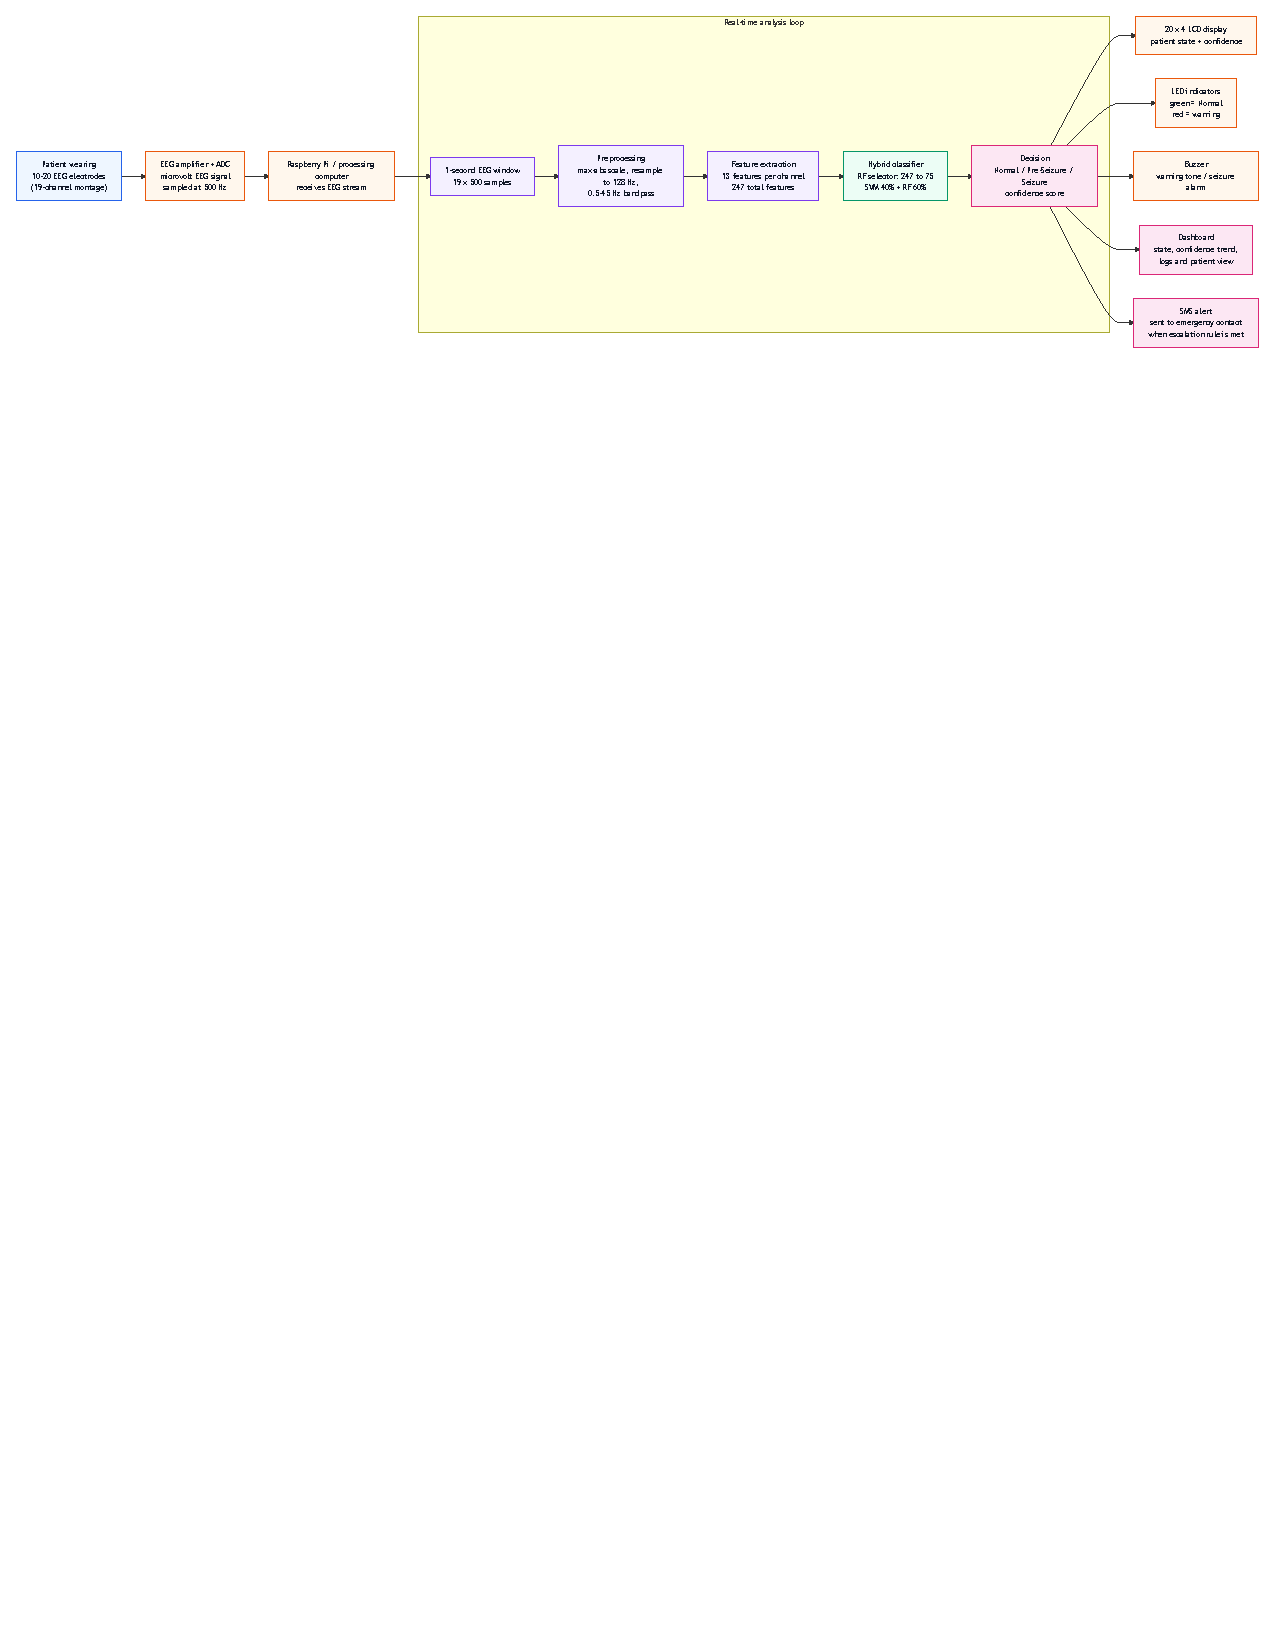
\includegraphics[
    width=0.88\textwidth,
    height=0.68\textheight,
    keepaspectratio
  ]{hardware_prototype_plan}
  \caption{Hardware prototype plan showing signal acquisition, digitisation,
           windowing, preprocessing, feature extraction, classification,
           and alert output with expected latency.}
  \label{fig:hardware_prototype_plan}
\end{figure}

Table~\ref{tab:hardware} lists all hardware components used in the prototype,
together with their GPIO pin assignments under the Broadcom (BCM) numbering scheme.

\begin{table}[H]
    \centering
    \caption{NeuroWatch Hardware Components and GPIO Configuration}
    \label{tab:hardware}
    \begin{tabular}{llll}
        \toprule
        \textbf{Component} & \textbf{Specification} & \textbf{GPIO Pin (BCM)} & \textbf{Purpose} \\
        \midrule
        Raspberry Pi        & Model 3B / 4B           & ---          & Main processing unit \\
        \midrule
        \multirow{5}{*}{LCD Display}
                            & 20$\times$4 Character   & RS: 26       & \multirow{5}{*}{Patient state display} \\
                            & HD44780 Controller      & E:  19       & \\
                            & 5V, Green backlight     & D4: 13       & \\
                            &                         & D5: 6        & \\
                            &                         & D6: 5, D7: 20& \\
        \midrule
        Red LED             & 5mm, 2V                 & GPIO 22      & Seizure / alert indicator \\
        Green LED           & 5mm, 2V                 & GPIO 27      & Normal state indicator \\
        Blue LED            & 5mm, 3V                 & ---          & Power / status indicator \\
        \midrule
        Buzzer              & Active, 5V              & GPIO 4       & Audible seizure alarm \\
        \midrule
        Resistors           & 220$\Omega$             & ---          & Current limiting for LEDs \\
        Breadboard          & 830-point               & ---          & Component interconnection \\
        Jumper Wires        & Male-to-female          & ---          & GPIO to breadboard wiring \\
        \bottomrule
    \end{tabular}
\end{table}

\subsection{Circuit Simulation}
\label{sec:simulation}

Before assembling the physical hardware, the NeuroWatch circuit was simulated
in \textbf{Proteus Design Suite} to validate the LCD display, LED indicators,
and buzzer behaviour under each patient state. This step ensured that the
software logic produced the correct visual and audible outputs before any
physical wiring was performed. Figures~\ref{fig:sim_startup}
to~\ref{fig:sim_seizure} show the simulation running through each system
state.

Table~\ref{tab:proteus_test_cases} links the Proteus screenshots to the
test cases used during simulation. Each case checks whether the simulated
LCD, LED, and buzzer outputs match the expected behaviour for that state.

\begin{table}[!htbp]
  \centering
  \caption{Proteus simulation test cases and observed outputs.}
  \label{tab:proteus_test_cases}
  \tiny
  \setlength{\tabcolsep}{3pt}
  \renewcommand{\arraystretch}{1.05}
  \begin{tabularx}{\textwidth}{>{\raggedright\arraybackslash}p{2.25cm}
                              >{\raggedright\arraybackslash}p{3.0cm}
                              >{\raggedright\arraybackslash}p{2.8cm}
                              >{\raggedright\arraybackslash}X
                              >{\centering\arraybackslash}p{0.9cm}}
    \toprule
    \textbf{Test case} & \textbf{Expected LCD output} & \textbf{LED / buzzer output} &
    \textbf{Observed Proteus output} & \textbf{Result} \\
    \midrule
    Startup &
    \texttt{NeuroWatch v1.3}; \texttt{System Booting..}; \texttt{Wait...} &
    Red LED OFF; buzzer OFF; heartbeat LED active &
    Startup screen displayed correctly with no alert output &
    Pass \\
    Waiting for model &
    \texttt{LCD READY}; \texttt{Waiting Model..} &
    Red LED OFF; buzzer OFF &
    LCD remained in waiting state until prediction opcodes arrived &
    Pass \\
    Normal state &
    Patient name; \texttt{STATE: Normal}; confidence; timestamp &
    Red LED OFF; buzzer OFF; heartbeat LED active &
    Normal display appeared with no warning output &
    Pass \\
    Pre-Seizure warning ($<12$ s) &
    Patient name; \texttt{STATE: Pre-Seizure}; confidence; timestamp &
    Red LED blinks; buzzer pulses &
    Warning state displayed and red indicator blinked &
    Pass \\
    Sustained Pre-Seizure ($\geq12$ s) &
    Patient name; \texttt{STATE: Pre-Seizure}; confidence; \texttt{TAKE MEDICATION} &
    Red LED blinks; buzzer pulses &
    Medication prompt appeared after sustained warning state &
    Pass \\
    Seizure alert ($<30$ s) &
    Blinking patient row; \texttt{STATE: Seizure}; confidence; timestamp &
    Red LED blinks; buzzer alarm active &
    Seizure state and alarm output appeared correctly &
    Pass \\
    Sustained Seizure ($\geq30$ s) &
    Blinking patient row; \texttt{STATE: Seizure}; confidence;
    \texttt{DR NOTIFIED} or \texttt{CONTACT DR} &
    Red LED blinks; buzzer alarm active &
    LCD escalated to notification message after the seizure timer threshold &
    Pass \\
    Restarting / model stopped &
    \texttt{RESTARTING}; \texttt{Please Wait...} &
    Red LED OFF; buzzer OFF &
    Circuit returned to a non-alert waiting state during restart &
    Pass \\
    \bottomrule
  \end{tabularx}
\end{table}

\begin{table}[!htbp]
  \centering
  \caption{Side-by-side comparison of simulated and hardware alert outputs.}
  \label{tab:simulation_hardware_outputs}
  \tiny
  \setlength{\tabcolsep}{3pt}
  \renewcommand{\arraystretch}{1.08}
  \begin{tabularx}{\textwidth}{>{\raggedright\arraybackslash}p{2.4cm}
                              >{\raggedright\arraybackslash}p{3.2cm}
                              >{\raggedright\arraybackslash}p{3.2cm}
                              >{\raggedright\arraybackslash}X}
    \toprule
    \textbf{Output device} & \textbf{Proteus simulation activity} &
    \textbf{Hardware prototype activity} & \textbf{Improvement verified} \\
    \midrule
    20$\times$4 LCD &
    Virtual LCD displayed startup, waiting, Normal, Pre-Seizure, Seizure,
    and notification screens &
    Physical HD44780 LCD displayed the same four-row format using GPIO &
    Confirmed that simulated display logic worked on a real LCD. \\
    Green LED &
    Simulated system-alive indicator &
    Physical green LED blinked as the heartbeat &
    Verified real GPIO status indication. \\
    Red LED &
    Simulated warning indicator during Pre-Seizure and Seizure &
    Physical red LED blinked during warning and alarm states &
    Confirmed alert-state GPIO switching. \\
    Buzzer &
    Simulated audible alert activation &
    Physical buzzer pulsed for Pre-Seizure and alarmed during Seizure &
    Verified real audible warning and alarm timing. \\
    Timed escalation &
    Proteus verified the 12-second \texttt{TAKE MEDICATION} and 30-second
    notification display logic &
    Hardware LCD displayed \texttt{TAKE MEDICATION}, \texttt{DR NOTIFIED},
    or \texttt{CONTACT DR} after the same timing thresholds &
    Confirmed that timers, display output, and alert peripherals stayed synchronised. \\
    \bottomrule
  \end{tabularx}
\end{table}

\begin{figure}[H]
    \centering
    \begin{subfigure}[b]{0.48\textwidth}
        \includegraphics[width=\textwidth]{SIMULATION STARTUP}
        \caption{Startup --- system initialising.}
        \label{fig:sim_startup}
    \end{subfigure}
    \hfill
    \begin{subfigure}[b]{0.48\textwidth}
        \includegraphics[width=\textwidth]{SIMULATION WAITING FOR MODEL}
        \caption{Waiting for model files to load.}
        \label{fig:sim_waiting}
    \end{subfigure}

    \vspace{0.6em}

    \begin{subfigure}[b]{0.48\textwidth}
        \includegraphics[width=\textwidth]{SIMULATION_NORMAL}
        \caption{Normal state --- green LED active.}
        \label{fig:sim_normal}
    \end{subfigure}
    \hfill
    \begin{subfigure}[b]{0.48\textwidth}
        \includegraphics[width=\textwidth]{SIMULATION_PRESEIZURE}
        \caption{Pre-Seizure --- red LED active, \textit{TAKE MEDICATION} prompt.}
        \label{fig:sim_preseizure}
    \end{subfigure}

    \vspace{0.6em}

    \begin{subfigure}[b]{0.48\textwidth}
        \includegraphics[width=\textwidth]{SIMULATION_SEIZURE}
        \caption{Seizure --- red LED and buzzer active.}
        \label{fig:sim_seizure}
    \end{subfigure}

    \caption{Proteus Design Suite simulation of the NeuroWatch circuit across
    all five system states. Each state is reflected on the 20$\times$4 LCD
    and the corresponding LED indicator.}
    \label{fig:simulation_all}
\end{figure}

\subsection{Hardware Prototype Demonstration}

The NeuroWatch hardware prototype was assembled on a breadboard connected to a
Raspberry Pi, incorporating a 20$\times$4 character LCD display, a red alert
LED, and a blue status LED. The system was validated end-to-end using the
Mendeley pre-ictal EEG dataset, confirming correct operation from EEG
classification through to physical output and remote SMS notification.

\subsubsection{System Startup}

Upon power-on, the monitoring engine performs a full LCD reset and displays a
startup message confirming the software version before entering the detection
loop.

\begin{figure}[H]
    \centering
    \includegraphics[width=0.6\textwidth]{Hardware_Pi_Startup}
    \caption{NeuroWatch LCD on startup displaying version and initialisation
    status prior to the detection loop.}
    \label{fig:lcd_startup}
\end{figure}

\subsubsection{Pre-Seizure Warning}

When the model detects a Pre-Seizure state sustained beyond 12 seconds, the
LCD displays a \textit{TAKE MEDICATION} prompt on the fourth row, alerting the
patient or caregiver to administer prescribed anti-epileptic medication before
a full seizure develops.

\begin{figure}[H]
    \centering
    \includegraphics[width=0.6\textwidth]{Hardware_Pi_Pre_Seizure}
    \caption{LCD displaying Pre-Seizure state at 47.8\% confidence with the
    \textit{TAKE MEDICATION} prompt after 12 seconds of sustained pre-ictal
    activity. The red LED is active as a visual warning.}
    \label{fig:lcd_preseizure}
\end{figure}

\subsubsection{Seizure Detection}

Upon Seizure classification, the red LED activates immediately and the LCD
updates to show the predicted state and model confidence. During the first
30 seconds, the fourth row displays the current timestamp while the system
monitors whether the state persists.

\begin{figure}[H]
    \centering
    \includegraphics[width=0.6\textwidth]{Hardware_Pi_Seizure}
    \caption{LCD displaying Seizure state at 80.7\% confidence within the
    30-second monitoring window. The timestamp on the fourth row indicates
    the system has not yet escalated to SMS notification.}
    \label{fig:lcd_seizure_early}
\end{figure}

\subsubsection{Sustained Seizure and Clinician Notification}

If the Seizure state persists continuously for 30 seconds, an SMS alert is
dispatched to the registered clinician via the Twilio API. The LCD fourth row
updates to \textit{DR NOTIFIED} or \textit{CONTACT DR} depending on whether
the message was successfully sent.

The 30-second SMS trigger is an engineering debounce threshold rather than a
clinical threshold taken from seizure-duration literature. Its purpose is to
reduce false alarms caused by isolated misclassified windows, transient
artefacts, or brief state fluctuations. Since predictions are produced once
per analysis cycle, requiring a sustained Seizure state ensures that SMS
notification is sent only when the alert persists long enough to justify
caregiver escalation. In this prototype, the threshold was selected to balance
responsiveness against false-positive notification risk.

\begin{figure}[H]
    \centering
    \begin{subfigure}[b]{0.48\textwidth}
        \includegraphics[width=\textwidth]{Hardware_Pi_DR_NOTIFIED}
        \caption{SMS successfully sent --- \textit{DR NOTIFIED} displayed
        at 70.2\% confidence.}
        \label{fig:lcd_drnotified}
    \end{subfigure}
    \hfill
    \begin{subfigure}[b]{0.48\textwidth}
        \includegraphics[width=\textwidth]{Hardware_Pi_NOTIFY_DR}
        \caption{SMS dispatch unconfirmed --- \textit{CONTACT DR} displayed
        at 73.2\% confidence.}
        \label{fig:lcd_contactdr}
    \end{subfigure}
    \caption{LCD output after 30 seconds of sustained Seizure state.
    The red LED remains active throughout the episode.}
    \label{fig:lcd_seizure_escalated}
\end{figure}

\subsubsection{SMS Alert Notifications}

Two SMS message types are dispatched via Twilio: a seizure alert after
30 seconds of sustained Seizure state, and a clearing message when the
patient's EEG returns to Normal following a confirmed episode.
Figure~\ref{fig:sms} shows received SMS messages confirming state recovery
for patient John Molebatsi (P001) across multiple test runs.

\begin{figure}[H]
    \centering
    \includegraphics[width=0.45\textwidth]{SMS_Notification}
    \caption{SMS messages received on the clinician's phone via Twilio
    confirming that patient John Molebatsi (P001, Neuro A) returned to Normal
    following detected seizure episodes. Each message includes the patient ID,
    ward, and timestamp of the state transition.}
    \label{fig:sms}
\end{figure}

\section{System Implementation}

\subsection{End-to-End System Flow}

Figure~\ref{fig:sysflow} shows the end-to-end data flow of the deployed
NeuroWatch system. Pre-processed EEG windows are fed into the feature
extraction pipeline, classified by the hybrid model, and the result is
simultaneously written to JSON (for the remote dashboard), displayed on the
20$\times$4 LCD via GPIO, and — when a sustained seizure is detected —
dispatched as an SMS alert via the Twilio API.

\begin{figure}[H]
\centering
\tikzset{
    process/.style  = {rectangle, rounded corners, minimum width=3.8cm,
                       minimum height=0.9cm, text centered, draw=black,
                       fill=blue!18, drop shadow},
    io/.style       = {trapezium, trapezium left angle=70,
                       trapezium right angle=110, minimum width=3.4cm,
                       minimum height=0.9cm, text centered, draw=black,
                       fill=orange!20, drop shadow},
    output/.style   = {rectangle, rounded corners, minimum width=3.8cm,
                       minimum height=0.9cm, text centered, draw=black,
                       fill=red!18, drop shadow},
    arrow/.style    = {thick,->,>=Stealth}
}
\begin{tikzpicture}[node distance=1.6cm]
    \node (input)   [io]      {\textbf{EEG Windows (.npy)}};
    \node (feat)    [process, below of=input]   {\textbf{Feature Extraction} \\ \small(19ch × 13 = 247 feats)};
    \node (sel)     [process, below of=feat]    {\textbf{RF Feature Selector} \\ \small(247 → 75 features)};
    \node (model)   [process, below of=sel]     {\textbf{Hybrid Model} \\ \small(SVM×0.40 + RF×0.60)};
    \node (pred)    [process, below of=model]   {\textbf{Predicted State + Confidence}};
    \node (lcd)     [output,  below left=1.2cm and 1.8cm of pred]  {\textbf{LCD / LED / Buzzer} \\ \small(GPIO — direct)};
    \node (json)    [output,  below of=pred]    {\textbf{JSON Files} \\ \small(Dashboard polling)};
    \node (sms)     [output,  below right=1.2cm and 1.8cm of pred] {\textbf{SMS Alert} \\ \small(Twilio, ≥30 s seizure)};

    \draw [arrow] (input) -- (feat);
    \draw [arrow] (feat)  -- (sel);
    \draw [arrow] (sel)   -- (model);
    \draw [arrow] (model) -- (pred);
    \draw [arrow] (pred)  -- (lcd);
    \draw [arrow] (pred)  -- (json);
    \draw [arrow] (pred)  -- (sms);
\end{tikzpicture}
\caption{NeuroWatch end-to-end system flow. Outputs branch to three
independent channels: GPIO hardware, JSON-based dashboard, and Twilio SMS.}
\label{fig:sysflow}
\end{figure}

\subsection{Dashboard Data Flow and Timing}

The dashboard screenshots shown in this chapter are generated from the same
file-based data path used by the monitoring engine. The dashboard does not
run a separate classifier and does not independently simulate prediction
states. Instead, the inference script produces the current state, confidence
score, alert status, and patient information, then writes these values to
runtime JSON files. The dashboard reads those JSON files and refreshes its
display at a fixed polling interval.

\begin{table}[H]
  \centering
  \caption{Dashboard data source and timing behaviour.}
  \label{tab:dashboard_data_timing}
  \footnotesize
  \renewcommand{\arraystretch}{1.18}
  \begin{tabularx}{\textwidth}{>{\raggedright\arraybackslash}p{3.2cm}
                              >{\raggedright\arraybackslash}p{4.5cm}
                              >{\raggedright\arraybackslash}X}
    \toprule
    \textbf{Item} & \textbf{Data source or timing} & \textbf{Explanation} \\
    \midrule
    Prediction interval &
    One prediction is produced every analysis cycle, approximately every
    1--2~s depending on file loading, feature extraction, and GPIO update time &
    Each cycle processes one EEG window, extracts features, applies the
    RF selector, and evaluates the SVM--RF ensemble. \\
    JSON status update &
    \texttt{neurowatch\_status.json} and
    \texttt{neurowatch\_patients.json} are updated once per prediction cycle &
    These files contain the latest patient state, confidence score, alert
    status, and patient metadata used by the dashboard. \\
    Dashboard refresh rate &
    The dashboard polls the runtime JSON files approximately every 30~s &
    The displayed state is near-real-time but may lag behind the inference
    loop by up to one dashboard refresh interval. \\
    Stored records &
    Patient records and model summary metrics are loaded from JSON files such
    as \texttt{neurowatch\_patients.json} and
    \texttt{neurowatch\_metrics.json} &
    These are stored project outputs, not manually typed dashboard values. \\
    SMS delay &
    SMS is not sent after a single Seizure prediction; it is sent only after
    30 continuous seconds of Seizure state, followed by Twilio network
    delivery time &
    The 30-second delay is an engineering debounce rule to reduce false SMS
    alerts from isolated misclassifications. \\
    Demonstration limitation &
    The prototype uses stored EEG windows from the reconstructed dataset
    rather than a live physical EEG sensor &
    The dashboard demonstrates live software data flow from inference to JSON
    and then to the interface, while physical EEG acquisition remains part of
    the proposed hardware deployment. \\
    \bottomrule
  \end{tabularx}
\end{table}

% ── Custom colours used by the tables below ─────────────────────────────────
\definecolor{headerblue}{RGB}{51,102,187}
\definecolor{lightgray}{RGB}{242,242,242}

%% ── TABLE: LCD Display Behaviour ────────────────────────────────────────────
\clearpage
\begin{landscape}
\subsection{LCD Display Behaviour}

\noindent Figure~\ref{fig:lcd_state_transition} links the LCD messages to
the classifier output, confidence-driven state changes, and time thresholds.
The state machine shows how the display moves from Normal to Pre-Seizure,
then to Seizure if the alert escalates, and finally to Recovery when the
model returns to Normal.

\begin{figure}[H]
  \centering
  
\includegraphics[
    width=0.98\linewidth,
    height=0.86\textheight,
    keepaspectratio
  ]{lcd_state_transition}
  \caption{LCD and alert state-transition diagram for Normal,
           Pre-Seizure, Seizure, and Recovery behaviour.}
  \label{fig:lcd_state_transition}
\end{figure}

\clearpage

\begin{table}[H]
\centering
\caption{Table 4.1: LCD Display Behavior (Raspberry Pi Code)}
\label{tab:lcd_behaviour}
\normalsize
\resizebox{\linewidth}{!}{%
\begin{tabular}{|p{2.6cm}|p{2.0cm}|p{3.2cm}|p{3.2cm}|p{3.0cm}|p{2.0cm}|p{2.0cm}|p{3.2cm}|}
\hline
\textbf{Hardware} & \textbf{Interactive} & \textbf{System} & \textbf{Boost} & \textbf{Display Timeline} & \textbf{OFF (LED)} & \textbf{OFF (Buzzer)} & \textbf{Initial Learning} \\
\hline

Startup &
1 s &
\texttt{NeuroWatch v1.3 / Wait...} &
(blank) &
Steady &
OFF &
OFF &
Loads pre-trained \texttt{.pkl} models from disk \\
\hline

\rowcolor{lightgray}
Load Error &
1 s &
\texttt{LOAD ERROR / Check /models} &
Error text (20 chars) &
Steady &
OFF &
OFF &
Engine halts; check model path \\
\hline

Normal &
2 s &
\texttt{STATE: Normal} &
\texttt{T:HH:MM:SS} &
Steady &
OFF (Red) &
OFF &
Green LED on; model classifies each window \\
\hline

\rowcolor{lightgray}
Pre-Seizure &
2 s &
\texttt{STATE: Pre-Seizure} &
\texttt{T:HH:MM:SS} &
Steady &
Blink (Red) &
OFF &
Red LED on; monitoring for 12-s threshold \\
\hline

Pre-Seizure (sustained $\geq$12 s) &
2 s &
\texttt{STATE: Pre-Seizure} &
\texttt{TAKE MEDICATION} &
Steady &
Blink (Red) &
Pulse (1 Hz) &
Row 4 escalates to medication prompt \\
\hline

\rowcolor{lightgray}
Seizure &
2 s &
\texttt{STATE: Seizure} &
\texttt{T:HH:MM:SS} &
Blink (continuous) &
Blink (Red) &
Buzzer ON (5 Hz) &
Monitoring 30-s escalation window \\
\hline

Seizure (SMS sent, $\geq$30 s) &
2 s &
\texttt{STATE: Seizure} &
\texttt{DR NOTIFIED} &
Blink (continuous) &
Blink (Red) &
Buzzer ON (5 Hz) &
Twilio alert dispatched; one alert per episode \\
\hline

\rowcolor{lightgray}
Seizure (SMS failed, $\geq$30 s) &
2 s &
\texttt{STATE: Seizure} &
\texttt{CONTACT DR} &
Blink (continuous) &
Blink (Red) &
Buzzer ON (5 Hz) &
SMS not delivered; caregiver notified manually \\
\hline

\end{tabular}
}
\end{table}
\end{landscape}

%% ── TABLE: ML Model Processing Pipeline ─────────────────────────────────────
\begin{landscape}
\subsection{ML Model Processing Pipeline}

\begin{table}[H]
\centering
\caption{Stages of the NeuroWatch ML processing pipeline during live
         monitoring.}
\label{tab:ml_pipeline}
\resizebox{\linewidth}{!}{%
\begin{tabular}{|p{3.2cm}|p{5.0cm}|p{5.5cm}|p{4.5cm}|}
\hline
\rowcolor{headerblue}
\textcolor{white}{\textbf{Stage}} &
\textcolor{white}{\textbf{Action}} &
\textcolor{white}{\textbf{Details}} &
\textcolor{white}{\textbf{Output}} \\
\hline

Model Loading &
\texttt{joblib.load()} for five \texttt{.pkl} files &
\texttt{scaler.pkl}, \texttt{svm\_model.pkl}, \texttt{rf\_model.pkl},
\texttt{selector.pkl} (75 features), \texttt{ensemble\_weights.pkl}
(SVM 40\,\%, RF 60\,\%) &
Pre-trained models ready; no runtime training \\
\hline

\rowcolor{lightgray}
Data Loading &
\texttt{numpy.load()} for \texttt{x\_train.npy} and \texttt{x\_test.npy} &
19-channel Mendeley EEG windows, 500\,Hz, pooled into $\sim$11\,685 samples &
\texttt{live\_samples} list \\
\hline

Background Metrics &
Compute accuracy, F1, recall on all samples in a daemon thread &
\texttt{sklearn} metrics; writes \texttt{neurowatch\_metrics.json} &
Dashboard Metrics tab populated \\
\hline

\rowcolor{lightgray}
Feature Extraction &
Per window: resample 500$\to$128\,Hz, bandpass 0.5–45\,Hz,
Welch PSD, Hjorth, stats $\times$ 19 channels &
5 band powers + 3 Hjorth + 5 statistical/spectral features per channel = 13 features $\times$ 19 = 247 total &
247-element feature vector \\
\hline

Feature Selection &
Apply \texttt{RFImportanceSelector} (bootstrap RF importance) &
247 features reduced to top 75 most informative for SVM input &
75-element feature vector \\
\hline

\rowcolor{lightgray}
Prediction &
SVM probability $\times$ 0.40 + RF probability $\times$ 0.60 $\to$ \texttt{argmax} &
Class 0 = Normal, 1 = Pre-Seizure, 2 = Seizure; confidence = winning probability &
Predicted class + confidence score \\
\hline

Output &
Write \texttt{neurowatch\_patients.json} and \texttt{neurowatch\_status.json};
update LCD via GPIO; set LED / buzzer level &
JSON updated every cycle ($\sim$2\,s); dashboard polls every 30\,s &
Real-time display + remote visibility \\
\hline

\rowcolor{lightgray}
SMS Alert &
If Seizure state persists $\geq$30\,s, call \texttt{send\_sms\_alert()} via Twilio API &
One alert per episode; clearing SMS sent when state returns to Normal &
SMS to registered clinician numbers \\
\hline

\end{tabular}
}
\end{table}
\end{landscape}

%% ── TABLE: System Communication Interfaces ──────────────────────────────────
\begin{landscape}
\subsection{System Communication Interfaces}

\begin{table}[H]
\centering
\caption{Communication interfaces used by the NeuroWatch monitoring engine.
         All hardware outputs are driven directly via Raspberry Pi GPIO ---
         no serial bridge or intermediate simulation layer is used.}
\label{tab:comm_interfaces}
\resizebox{\linewidth}{!}{%
\begin{tabular}{|p{2.8cm}|p{3.0cm}|p{2.5cm}|p{3.5cm}|p{4.5cm}|}
\hline
\rowcolor{headerblue}
\textcolor{white}{\textbf{Interface}} &
\textcolor{white}{\textbf{Connection}} &
\textcolor{white}{\textbf{Direction}} &
\textcolor{white}{\textbf{Protocol}} &
\textcolor{white}{\textbf{Behaviour}} \\
\hline

LCD 20$\times$4 &
GPIO RS=26, E=19, D4–D7=13,6,5,20 &
Engine $\to$ LCD &
4-bit parallel (HD44780) &
Updated each prediction cycle; startup reset clears ghost characters \\
\hline

\rowcolor{lightgray}
Green LED &
GPIO 27 (digital out) &
Engine $\to$ LED &
Digital HIGH / LOW &
HIGH (on) when state = Normal; OFF otherwise \\
\hline

Red LED &
GPIO 22 (digital out) &
Engine $\to$ LED &
Digital HIGH / LOW &
HIGH (on) when state = Pre-Seizure or Seizure; OFF when Normal \\
\hline

\rowcolor{lightgray}
Buzzer &
GPIO 4 (PWM) &
Buzzer thread $\to$ Buzzer &
Software PWM (background thread) &
Silent for Normal; 0.18\,s pulse per second for Pre-Seizure;
5\,Hz square wave for Seizure \\
\hline

Dashboard &
\texttt{json/neurowatch\_patients.json} &
Engine $\to$ File $\to$ Dashboard &
File I/O (JSON) &
Engine writes each cycle; Streamlit dashboard reads and refreshes every 30\,s \\
\hline

\rowcolor{lightgray}
SMS Notification &
Twilio REST API (HTTPS) &
Engine $\to$ Internet $\to$ Phone &
HTTP POST via \texttt{twilio} library &
Seizure alert after 30\,s sustained Seizure; clearing alert on return to Normal \\
\hline

\end{tabular}
}
\end{table}
\end{landscape}

\subsection{Hardware Pin Configuration}

\begin{table}[H]
\centering
\caption{Raspberry Pi GPIO pin mapping (BCM numbering) for all NeuroWatch
         hardware peripherals.}
\label{tab:pinconfig}
\begin{tabular}{|l|c|l|}
\hline
\rowcolor{headerblue}
\textcolor{white}{\textbf{Component}} &
\textcolor{white}{\textbf{GPIO Pin (BCM)}} &
\textcolor{white}{\textbf{Purpose}} \\
\hline
LCD RS       & 26          & Register Select \\
\hline
\rowcolor{lightgray}
LCD E        & 19          & Enable \\
\hline
LCD D4–D7    & 13, 6, 5, 20 & 4-bit data lines \\
\hline
\rowcolor{lightgray}
Green LED    & 27          & Normal state indicator (ON = Normal) \\
\hline
Red LED      & 22          & Alert indicator (ON = Pre-Seizure or Seizure) \\
\hline
\rowcolor{lightgray}
Buzzer       & 4           & Audible alarm (pulsed for Pre-Seizure; 5\,Hz for Seizure) \\
\hline
\end{tabular}
\end{table}

%% ============================================================
\chapter{Results and Discussion}
%% ============================================================

\section{Overview of Trained Models}

Four model configurations were trained and evaluated sequentially, each
building on the lessons learned from the previous iteration. Table~\ref{tab:allmodels}
summarises their performance on the held-out test set.

\begin{table}[H]
  \centering
  \caption{Comparative test-set performance of all trained model configurations.
           Seizure Recall and Overfitting Gap are key evaluation indicators.}
  \label{tab:allmodels}
  \begin{tabular}{lcccccc}
    \toprule
    \textbf{Model} & \textbf{Acc.} & \textbf{F1} & \textbf{Prec.}
                   & \textbf{Sz. Recall} & \textbf{OFit Gap} & \textbf{$\theta$} \\
    \midrule
    MODELS\_V1 (ANOVA sel.)        & 72.5\% & 72.0\% & 72.3\% & 78.0\% & 14.2\% & --- \\
    MODELS\_FS75 (RF sel., C=1)    & 76.1\% & 75.8\% & 76.0\% & 85.1\% & 5.9\%  & 0.42 \\
    RF60+SVM40 (RF sel., C=1)      & 75.0\% & 74.8\% & 75.1\% & 84.9\% & 6.3\%  & 0.37 \\
    \textbf{RF60+SVM40\_C2 (final)}& \textbf{77.07\%} & \textbf{77.12\%} & \textbf{77.2\%}
                                   & \textbf{86.67\%} & \textbf{6.8\%} & \textbf{0.39} \\
    \bottomrule
  \end{tabular}
\end{table}

The final RF60+SVM40\_C2 model therefore achieves
\textbf{promising prototype-level performance}: 77.07\% test accuracy,
77.12\% weighted F1-score, and 86.67\% Seizure recall. These values are
acceptable for an engineering prototype and demonstrate that the proposed
feature-engineering and hybrid-classifier pipeline is viable. However, they
should not be interpreted as evidence of deployment readiness. Additional
patient-level validation, continuous-recording false-alarm analysis, and
testing on live EEG hardware would be required before any operational use.

\begin{figure}[H]
  \centering
  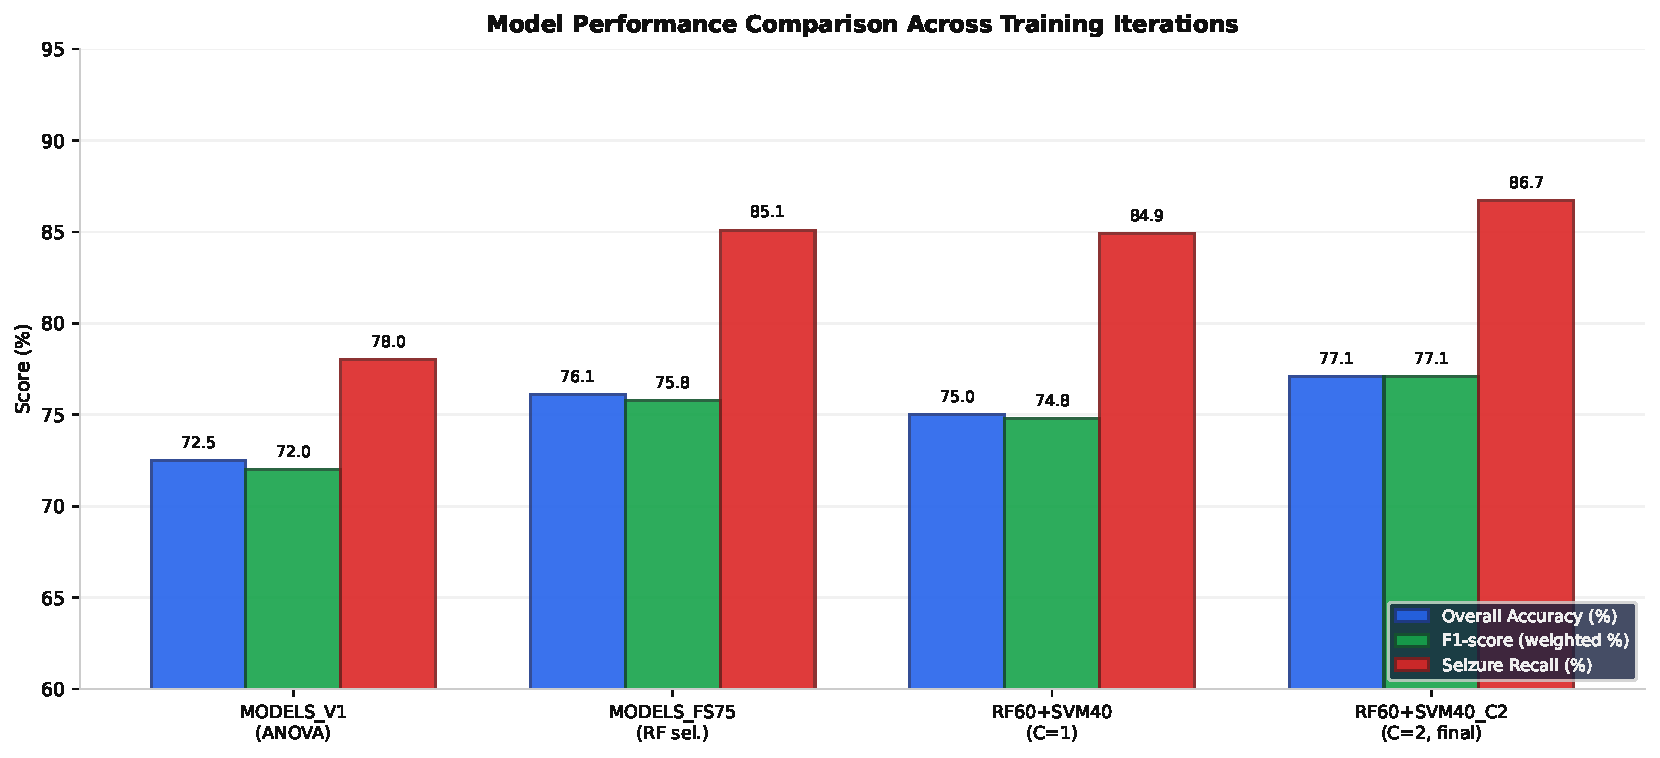
\includegraphics[width=0.92\linewidth]{fig5_results_comparison}
  \caption{Bar chart comparing overall accuracy, weighted F1-score, and
           seizure recall across all four model iterations. The final
           RF60+SVM40\_C2 model achieves the best performance on all
           three metrics.}
  \label{fig:comparison}
\end{figure}

\section{Confusion Matrix Analysis}

The confusion matrix of the final RF60+SVM40\_C2 model (Figure~\ref{fig:cm})
reveals the classification behaviour across all three classes.

\begin{figure}[H]
  \centering
  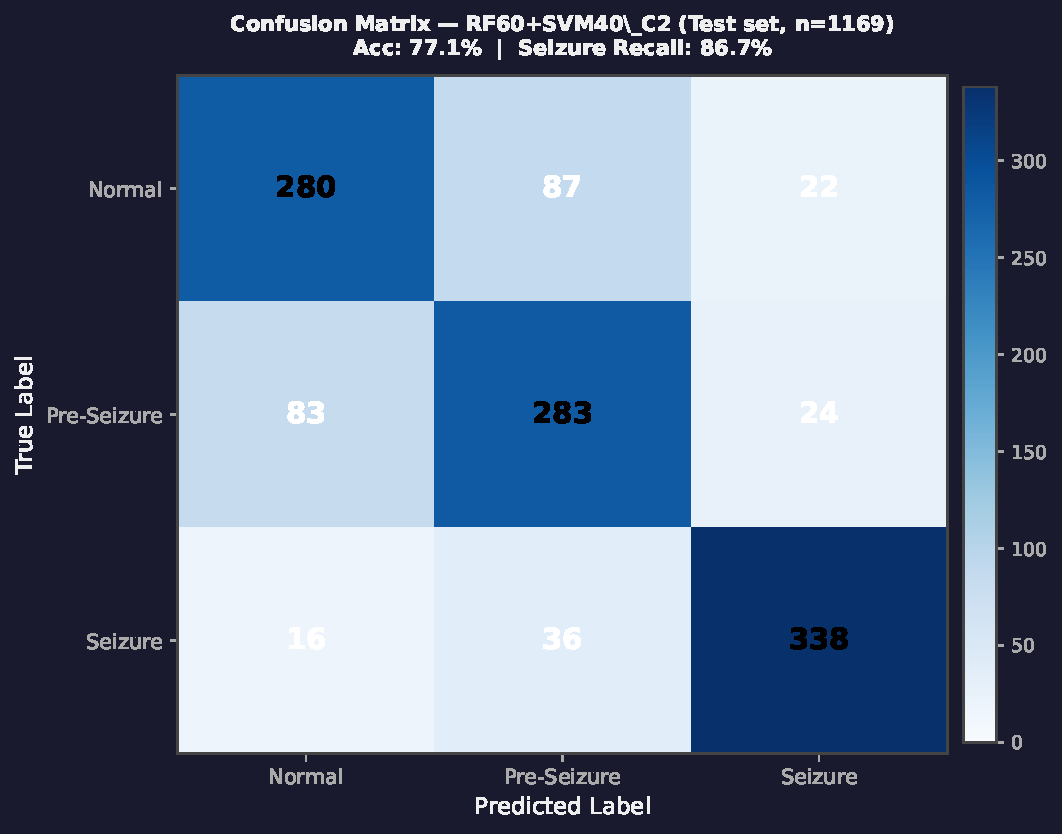
\includegraphics[width=0.65\linewidth]{fig6_confusion_matrix}
  \caption{Test-set confusion matrix for the final RF60+SVM40\_C2 model
           ($n=1{,}169$ samples). Rows correspond to true labels; columns
           to predicted labels.}
  \label{fig:cm}
\end{figure}

\begin{table}[H]
  \centering
  \caption{Per-class precision, recall, and F1-score for RF60+SVM40\_C2.}
  \label{tab:perclass}
  \begin{tabular}{lcccc}
    \toprule
    \textbf{Class} & \textbf{Count} & \textbf{Precision} & \textbf{Recall} & \textbf{F1} \\
    \midrule
    Normal      & 389 & 0.739 & 0.720 & 0.729 \\
    Pre-Seizure & 390 & 0.697 & 0.726 & 0.711 \\
    Seizure     & 390 & 0.880 & 0.867 & 0.873 \\
    \midrule
    \textbf{Weighted avg.} & 1{,}169 & \textbf{0.772} & \textbf{0.771} & \textbf{0.771} \\
    \bottomrule
  \end{tabular}
\end{table}

The Seizure class achieves the highest recall (86.67\%) and precision
(88.0\%), making it the most consistently detected class in the prototype test set.
Only 52 of 390 true Seizure windows were misclassified: 16 as Normal and
36 as Pre-Seizure. The Pre-Seizure class is the most challenging,
exhibiting the lowest F1-score (0.711). Since early warning depends on
detecting Pre-Seizure windows reliably, these errors require more detailed
interpretation than the overall accuracy alone.

\begin{table}[H]
  \centering
  \caption{Test-set error analysis for the final RF60+SVM40\_C2 model.}
  \label{tab:error_analysis}
  \small
  \renewcommand{\arraystretch}{1.15}
  \begin{tabularx}{\textwidth}{>{\raggedright\arraybackslash}p{3.3cm}
                              >{\centering\arraybackslash}p{2.1cm}
                              >{\raggedright\arraybackslash}X}
    \toprule
    \textbf{Error type} & \textbf{Windows} & \textbf{Engineering interpretation} \\
    \midrule
    Pre-Seizure predicted as Normal &
    83 &
    Most important early-warning error because a warning window is missed
    and no patient prompt is produced. \\
    Pre-Seizure predicted as Seizure &
    24 &
    Produces a stronger-than-needed alert, which is safer than missing the
    event but may increase alarm burden. \\
    Normal predicted as Pre-Seizure &
    87 &
    Creates false warning prompts and may contribute to alarm fatigue if it
    occurs repeatedly in continuous monitoring. \\
    Normal predicted as Seizure &
    22 &
    Most disruptive false alarm type because it can trigger seizure-level
    alert behaviour if sustained. \\
    Seizure predicted as Normal &
    16 &
    Critical missed-seizure error; future temporal smoothing should reduce
    isolated missed windows. \\
    Seizure predicted as Pre-Seizure &
    36 &
    Underestimates the severity but still keeps the system in an alert state. \\
    \bottomrule
  \end{tabularx}
\end{table}

From an engineering perspective, false Normal predictions during
Pre-Seizure or Seizure windows are the highest-risk errors because they
delay or suppress alerts. Conversely, false Pre-Seizure predictions during
Normal windows mainly create alarm fatigue. This trade-off explains why the
model emphasises Seizure recall and why future work should add temporal
smoothing over consecutive predictions rather than relying on isolated
one-second windows.

\section{Impact of the RF Importance Selector}

Replacing the ANOVA F-score SelectKBest with the bootstrap RF importance
selector produced a \textbf{3.6 percentage-point increase} in overall
accuracy (72.5\% $\to$ 76.1\%) and a \textbf{7.1 percentage-point increase}
in seizure recall (78.0\% $\to$ 85.1\%) when moving from MODELS\_V1 to
MODELS\_FS75. The RF importance measure captures non-linear interactions
between features that ANOVA F-score, which assumes linear separability,
cannot exploit. Furthermore, the overfitting gap fell from 14.2\% to 5.9\%,
indicating that the RF-selected features generalise substantially better.

\section{Effect of Increasing SVM Regularisation ($C$: 1 $\to$ 2)}

Increasing the SVM penalty parameter from $C=1$ to $C=2$ tightened the
decision boundary, yielding a 1.0 percentage-point accuracy improvement
(76.1\% $\to$ 77.1\%) and a 1.6 percentage-point seizure recall improvement
(85.1\% $\to$ 86.7\%). The overfitting gap increased slightly from 5.9\%
to 6.8\%, which remains within an acceptable range ($<10\%$). This suggests
that the dataset is sufficiently large to support a slightly less-regularised
SVM without significant overfitting.

\section{Ensemble Weight Analysis}

The final ensemble weights ($\alpha_{\text{SVM}}=0.40$,
$\alpha_{\text{RF}}=0.60$) were determined by a validation-set grid search
across the full $[0.0, 1.0]$ range. In preliminary experiments with a
highly constrained RF (\texttt{max\_depth=5}, \texttt{min\_samples\_leaf=10}),
the auto-tuner consistently assigned SVM weights above 90\%, because the
underpowered RF contributed very little discriminative signal. After
increasing the RF capacity (\texttt{max\_depth=8}, \texttt{min\_samples\_leaf=4}),
the RF became competitive, and the optimiser converged to the balanced
40/60 split. This demonstrates that ensemble diversity---achieved by
allowing both base learners to perform competitively---is important for
optimal blending.

\section{Normal Threshold Correction Effect}

The tuned threshold $\theta=0.39$ means that a Pre-Seizure prediction is
overridden to Normal whenever the combined model assigns at least 39\%
probability to the Normal class. This low threshold reflects the tendency
of the uncorrected ensemble to predict Pre-Seizure on ambiguous windows
that are likely Normal. By applying the correction on the validation set,
the precision of the Normal class improved without any adverse effect on
seizure recall (the correction is never applied when the argmax is Seizure).

\section{Class Weight Analysis}

Assigning a class weight of 1.8 to the Pre-Seizure class in the SVM
training penalises misclassification of Pre-Seizure samples at 1.8$\times$
the cost of Normal or Seizure misclassifications. This directly improved
Pre-Seizure recall from approximately 67\% (equal weights) to 72.6\%
in the final model. The trade-off is a small reduction in Normal precision,
which is partially compensated by the threshold correction.

\section{Overfitting Analysis}

The overfitting gap, defined as the difference between training and test
accuracy, decreased substantially as the feature selector was improved:
from 14.2\% (ANOVA) to 5.9\% (RF selector). A gap below 10\% is generally
considered acceptable for a model of this complexity. The residual gap of
6.8 percentage points in the final model is attributable to the small patient cohort (6
patients), which limits the diversity of training examples, rather than
to architectural over-complexity.

\section{Operational Prototype Metrics}

Table~\ref{tab:operational_metrics} reports system-level metrics that are
important for the prototype objective but are not captured by accuracy and
F1-score alone.

\begin{table}[H]
  \centering
  \caption{Operational metrics for the prototype monitoring pipeline.}
  \label{tab:operational_metrics}
  \small
  \renewcommand{\arraystretch}{1.15}
  \begin{tabularx}{\textwidth}{>{\raggedright\arraybackslash}p{4.2cm}
                              >{\raggedright\arraybackslash}p{3.8cm}
                              >{\raggedright\arraybackslash}X}
    \toprule
    \textbf{Metric} & \textbf{Prototype value} & \textbf{Interpretation} \\
    \midrule
    Inference interval per window &
    Approximately 1--2~s per analysis cycle &
    Includes feature extraction, RF selection, SVM/RF prediction, JSON update,
    and hardware-output refresh. \\
    Mean detection latency &
    Approximately one analysis cycle after a window is processed &
    The classifier produces a decision once the current one-second EEG window
    has been analysed. \\
    SMS delay &
    30~s sustained Seizure state plus Twilio network delivery time &
    SMS delay is intentionally added as an engineering debounce rule to reduce
    false notifications. \\
    Dashboard refresh rate &
    Approximately 30~s &
    The dashboard polls JSON outputs periodically; the LCD and JSON status
    files update more frequently than the dashboard display. \\
    False alarm rate per hour &
    Not validly estimated from the balanced test split &
    The held-out test set is balanced and window-based, not a continuous
    chronological EEG stream. As a surrogate, 109 of 389 Normal test windows
    were classified as Pre-Seizure or Seizure. A true false-alarm/hour metric
    requires continuous-recording evaluation. \\
    \bottomrule
  \end{tabularx}
\end{table}

\section{Comparison with Literature and Task Scope}

Direct comparison with published EEG seizure-detection studies must be made
carefully because reported results often use different datasets, class
definitions, patient splits, and evaluation tasks. Table~\ref{tab:literature_scope}
therefore separates task type from headline performance.

\begin{table}[H]
  \centering
  \caption{Task-scope comparison for interpreting reported performance.}
  \label{tab:literature_scope}
  \small
  \renewcommand{\arraystretch}{1.15}
  \begin{tabularx}{\textwidth}{>{\raggedright\arraybackslash}p{3.2cm}
                              >{\raggedright\arraybackslash}p{3.8cm}
                              >{\raggedright\arraybackslash}p{3.2cm}
                              >{\raggedright\arraybackslash}X}
    \toprule
    \textbf{Study/model type} & \textbf{Task type} & \textbf{Evaluation setting} & \textbf{Comparability note} \\
    \midrule
    Binary seizure detectors &
    Seizure vs non-seizure detection &
    Often easier two-class separation &
    Not directly comparable with this project's three-class Normal,
    Pre-Seizure, and Seizure formulation. \\
    Patient-specific predictors &
    Prediction horizon or patient-specific warning &
    May train and test separately per patient &
    Can achieve higher performance because inter-patient variation is reduced. \\
    Deep learning baselines &
    Binary or multiclass seizure detection &
    Often require larger datasets and more compute &
    Useful as performance context but not identical to the lightweight
    edge-deployable prototype objective. \\
    This project &
    Three-class prototype detection: Normal, Pre-Seizure, Seizure &
    Reconstructed EDF-based Mendeley corpus with 80/10/10 split &
    Reported results should be interpreted as promising prototype-level
    performance, not deployment-ready evidence. \\
    \bottomrule
  \end{tabularx}
\end{table}

\section{Discussion}

The results demonstrate that a handcrafted feature engineering approach,
combined with a hybrid SVM+RF ensemble, can achieve useful
prototype-level seizure detection performance on a challenging multi-class
EEG dataset. The 86.67\% Seizure recall is important from an engineering
safety perspective because missed Seizure windows reduce the chance of a
timely alert, while false alerts can contribute to alarm fatigue.

Several limitations of the current approach are noted:

\begin{enumerate}
  \item \textbf{Patient-independent evaluation}: The train/test split is
        performed across the pooled patient data rather than across
        patients, which may inflate apparent generalisation. A
        leave-one-patient-out evaluation would provide a stricter bound.
  \item \textbf{Small cohort}: Six patients is insufficient to capture
        the full inter-patient variability of EEG morphology in focal
        epilepsy.
  \item \textbf{Fixed window size}: The one-second window may miss
        slow pre-ictal build-up patterns that span several seconds.
  \item \textbf{No temporal context}: The classifier treats each window
        independently, ignoring sequential state transitions that could
        reduce false alarms.
\end{enumerate}

%% ============================================================
\chapter{Conclusion}
%% ============================================================

\section{Summary of Contributions}

This project designed, implemented, and evaluated a complete
remote EEG seizure detection pipeline targeting deployment on a Raspberry
Pi 4 edge device. The key engineering contributions are:

\begin{itemize}
  \item A \textbf{modular feature extraction pipeline} computing 247
        handcrafted features per one-second EEG window, covering spectral,
        temporal, and nonlinear domains.
  \item A \textbf{bootstrap RF importance feature selector}
        (\texttt{RFImportanceSelector}) that uses Random Forest for
        feature ranking and selection, outperforming ANOVA F-score
        SelectKBest by capturing non-linear feature interactions.
  \item A \textbf{hybrid SVM+RF ensemble} in which Random Forest is also
        used as a classifier, contributing 60\% of the final ensemble
        probability against 40\% from the SVM, with a post-hoc Normal
        threshold correction that reduces
        false Pre-Seizure alarms without degrading seizure recall.
  \item A \textbf{real-time remote monitoring dashboard}
        (\texttt{dashboard\_v2.py}) displaying live EEG, classification
        state, patient records, and model metrics over a local network.
  \item A \textbf{reproducible training pipeline} with automatic model
        artefact saving, metrics export to \texttt{neurowatch\_metrics.json},
        and confusion matrix visualisation.
\end{itemize}

The final RF60+SVM40\_C2 model achieves \textbf{77.07\% overall accuracy},
\textbf{77.12\% weighted F1-score}, and \textbf{86.67\% Seizure recall}
on a balanced three-class dataset with a train/test overfitting gap of
\textbf{6.8 percentage points}. These results represent promising
prototype-level performance rather than deployment readiness.

\section{Conclusions}

The proposed system demonstrates that resource-constrained edge hardware can host an
EEG seizure detection prototype using classical machine learning.
The system successfully differentiates Normal, Pre-Seizure, and Seizure
brain states in near real-time, enabling a caregiver or clinician to
monitor a patient remotely and receive timely alerts without requiring
continuous EEG review.

The combination of RF importance-based feature selection with an asymmetric
SVM and a calibrated threshold correction proved superior to a single
classifier or an untuned ensemble. These findings confirm that careful
post-processing and class-imbalance handling are as important as
model architecture in EEG signal classification prototypes.

%% ============================================================
\chapter{Future Works}
%% ============================================================

\section{Short-Term Improvements}

\begin{enumerate}
  \item \textbf{Leave-one-patient-out cross-validation}: Evaluate the model
        strictly across patients to quantify inter-patient generalisation
        before any operational deployment.

  \item \textbf{Expanded feature set}: Incorporate inter-channel
        coherence features---the $\binom{19}{2}=171$ pairwise correlation
        coefficients---to capture network-level synchrony changes that
        precede seizures.

  \item \textbf{Temporal smoothing}: Apply a sliding majority vote or
        hidden Markov model (HMM) over consecutive window predictions to
        suppress isolated false alarms caused by transient artefacts.

  \item \textbf{Automated artefact rejection}: Add an upstream binary
        artefact detector (e.g., eye-blink and muscle contamination
        classifier) to gate the seizure detector, reducing false alarms
        in ambulatory settings.

  \item \textbf{Larger $C$ sweep / grid search}: Perform a broader
        SVM hyper-parameter search ($C \in [1, 10]$, $\gamma \in$
        \{scale, auto, 0.001, 0.01\}) with cross-validation to find the
        global optimum rather than a single incremental adjustment.
\end{enumerate}

\section{Medium-Term Directions}

\begin{enumerate}
  \item \textbf{Deep learning baseline}: Train a 1-D CNN or LSTM on the
        raw EEG signals to serve as a benchmark against the handcrafted
        pipeline. Temporal convolutional networks (TCNs) are particularly
        suited to EEG due to their ability to model long-range temporal
        dependencies.

  \item \textbf{Transfer learning}: Pre-train a feature extractor on a
        large public EEG dataset (e.g., Temple University Hospital Corpus)
        and fine-tune on the Mendeley dataset to overcome the small-cohort
        limitation.

  \item \textbf{Online adaptation}: Implement a lightweight online
        learning module that updates the Normal class boundary using
        confirmed normal windows from the deployed patient, personalising
        the detector to their baseline EEG.

  \item \textbf{Network communication layer}: Add an MQTT or WebSocket
        broker so that alerts are pushed to a caregiver's smartphone
        in real time over a hospital Wi-Fi or 4G network, completing
        the remote monitoring loop.
\end{enumerate}

\section{Long-Term Vision}

The long-term vision for NeuroWatch is a \textbf{fully autonomous,
wearable, patient-adaptive seizure monitoring system}. This requires:

\begin{itemize}
  \item Integration with a low-power, wearable EEG headset (dry electrodes,
        Bluetooth Low Energy) for ambulatory use outside the clinic.
  \item A cloud-based patient data store enabling longitudinal tracking
        of seizure frequency, duration, and morphology for neurologist review.
  \item Personalised threshold adaptation using reinforcement learning
        from clinician-confirmed and -rejected alerts.
  \item Regulatory compliance with IEC~62304 (medical device software
        lifecycle) and ISO~14971 (risk management) prior to any clinical
        deployment.
\end{itemize}

%% ── Bibliography ────────────────────────────────────────────
\begin{thebibliography}{99}

\bibitem{mendeley_dataset}
Ihle, M., Feldwisch-Drentrup, H., Teixeira, C.~A., Witon, A., Schelter, B.,
Timmer, J., \& Schulze-Bonhage, A. (2012).
\textit{EPILEPSIAE -- A European epilepsy database.}
Computer Methods and Programs in Biomedicine, 106(3), 127--138.

\bibitem{hjorth1970eeg}
Hjorth, B. (1970).
\textit{EEG analysis based on time domain properties.}
Electroencephalography and Clinical Neurophysiology, 29(3), 306--310.

\bibitem{welch1967power}
Welch, P. D. (1967).
\textit{The use of fast Fourier transform for the estimation of power
spectra: a method based on time averaging over short, modified periodograms.}
IEEE Transactions on Audio and Electroacoustics, 15(2), 70--73.

\bibitem{cortes1995svm}
Cortes, C., \& Vapnik, V. (1995).
\textit{Support-vector networks.}
Machine Learning, 20(3), 273--297.

\bibitem{platt1999svm}
Platt, J. (1999).
\textit{Probabilistic outputs for support vector machines and comparisons to
regularized likelihood methods.}
Advances in Large Margin Classifiers, 10(3), 61--74.

\bibitem{breiman2001rf}
Breiman, L. (2001).
\textit{Random forests.}
Machine Learning, 45(1), 5--32.

\bibitem{shoeb2004seizure}
Shoeb, A., \& Guttag, J. (2010).
\textit{Application of machine learning to epileptic seizure detection.}
Proceedings of the 27th International Conference on Machine Learning (ICML).

\end{thebibliography}

\end{document}
